\documentclass[english,floatsintext,man]{apa6}

\usepackage{amssymb,amsmath}
\usepackage{ifxetex,ifluatex}
\usepackage{fixltx2e} % provides \textsubscript
\ifnum 0\ifxetex 1\fi\ifluatex 1\fi=0 % if pdftex
  \usepackage[T1]{fontenc}
  \usepackage[utf8]{inputenc}
\else % if luatex or xelatex
  \ifxetex
    \usepackage{mathspec}
    \usepackage{xltxtra,xunicode}
  \else
    \usepackage{fontspec}
  \fi
  \defaultfontfeatures{Mapping=tex-text,Scale=MatchLowercase}
  \newcommand{\euro}{€}
\fi
% use upquote if available, for straight quotes in verbatim environments
\IfFileExists{upquote.sty}{\usepackage{upquote}}{}
% use microtype if available
\IfFileExists{microtype.sty}{\usepackage{microtype}}{}

% Table formatting
\usepackage{longtable, booktabs}
\usepackage{lscape}
% \usepackage[counterclockwise]{rotating}   % Landscape page setup for large tables
\usepackage{multirow}		% Table styling
\usepackage{tabularx}		% Control Column width
\usepackage[flushleft]{threeparttable}	% Allows for three part tables with a specified notes section
\usepackage{threeparttablex}            % Lets threeparttable work with longtable

% Create new environments so endfloat can handle them
% \newenvironment{ltable}
%   {\begin{landscape}\begin{center}\begin{threeparttable}}
%   {\end{threeparttable}\end{center}\end{landscape}}

\newenvironment{lltable}
  {\begin{landscape}\begin{center}\begin{ThreePartTable}}
  {\end{ThreePartTable}\end{center}\end{landscape}}




% The following enables adjusting longtable caption width to table width
% Solution found at http://golatex.de/longtable-mit-caption-so-breit-wie-die-tabelle-t15767.html
\makeatletter
\newcommand\LastLTentrywidth{1em}
\newlength\longtablewidth
\setlength{\longtablewidth}{1in}
\newcommand\getlongtablewidth{%
 \begingroup
  \ifcsname LT@\roman{LT@tables}\endcsname
  \global\longtablewidth=0pt
  \renewcommand\LT@entry[2]{\global\advance\longtablewidth by ##2\relax\gdef\LastLTentrywidth{##2}}%
  \@nameuse{LT@\roman{LT@tables}}%
  \fi
\endgroup}


\ifxetex
  \usepackage[setpagesize=false, % page size defined by xetex
              unicode=false, % unicode breaks when used with xetex
              xetex]{hyperref}
\else
  \usepackage[unicode=true]{hyperref}
\fi
\hypersetup{breaklinks=true,
            pdfauthor={},
            pdftitle={How social contexts shape active learning},
            colorlinks=true,
            citecolor=blue,
            urlcolor=blue,
            linkcolor=black,
            pdfborder={0 0 0}}
\urlstyle{same}  % don't use monospace font for urls

\setlength{\parindent}{0pt}
%\setlength{\parskip}{0pt plus 0pt minus 0pt}

\setlength{\emergencystretch}{3em}  % prevent overfull lines

\ifxetex
  \usepackage{polyglossia}
  \setmainlanguage{}
\else
  \usepackage[english]{babel}
\fi

% Manuscript styling
\captionsetup{font=singlespacing,justification=justified}
\usepackage{csquotes}
\usepackage{upgreek}



\usepackage{tikz} % Variable definition to generate author note

% fix for \tightlist problem in pandoc 1.14
\providecommand{\tightlist}{%
  \setlength{\itemsep}{0pt}\setlength{\parskip}{0pt}}

% Essential manuscript parts
  \title{How social contexts shape active learning}

  \shorttitle{Active learning is social}


  \author{Kyle MacDonald\textsuperscript{1}}

  \def\affdep{{""}}%
  \def\affcity{{""}}%

  \affiliation{
    \vspace{0.5cm}
          \textsuperscript{1} Stanford University  }

  \authornote{
    \newcounter{author}
    Conceptual Analysis of Dissertation Area.
    
    Readers: Michael C. Frank, Hyowon Gweon, and Anne Fernald

                        }


  \abstract{Children's rapid conceptual development is one of the more remarkable
features of human cognition. How do they learn so much so quickly?
Social learning theories argue for the importance of learning from rich
input provided by more knowledgeable others. In contrast, active
learning accounts focus on children's efficient information seeking
skills as a path to knowledge acquisition via self-directed exploration.
In this paper, I argue that an important step towards a complete theory
of early learning is to understand how active learning behaviors unfold
within social learning contexts. To integrate the two theoretical
accounts, I use the theory of Optimal Experiment Design (OED), which
formalizes human inquiry as a process of expected utility maximization
with respect to the goal of gaining new information. The heart of my
argument is that in order to characterize the usefulness of active
learning behaviors (e.g., causal interventions, eye movements, and
verbal question-asking) we must consider recent insights into how
decisions and learning are shaped by our interactions with other people.}
  \keywords{active learning, social learning, decision making, theory \\

    \indent Word count: X
  }





\usepackage{amsthm}
\newtheorem{theorem}{Theorem}
\newtheorem{lemma}{Lemma}
\theoremstyle{definition}
\newtheorem{definition}{Definition}
\newtheorem{corollary}{Corollary}
\newtheorem{proposition}{Proposition}
\theoremstyle{definition}
\newtheorem{example}{Example}
\theoremstyle{definition}
\newtheorem{exercise}{Exercise}
\theoremstyle{remark}
\newtheorem*{remark}{Remark}
\newtheorem*{solution}{Solution}
\begin{document}

\maketitle

\setcounter{secnumdepth}{0}



\section{Introduction}\label{introduction}

Human learning is remarkable. Consider that children, despite their
limitations on general processing capabilities, are able to acquire new
lexical concepts at a high rate, eventually reaching an adult vocabulary
ranging between 50,000 to 100,000 words (P. Bloom, 2002). And they
accomplish this all while also developing motor skills, learning social
norms, and building causal knowledge. How can we explain children's
prodigious learning abilities?

Social learning accounts offer a solution by pointing out that children
do not solve these problems on their own. Instead, children are
typically surrounded by parents, other knowledgeable adults, or older
peers -- all of whom likely know more than they do and are interested in
facilitating their learning. Social learning accounts also emphasize
that social contexts can bootstrap children's learning via several
mechanisms. For example, work on early language acquisition shows that
social partners provide input that is tuned to children's cognitive
abilities (Eaves Jr, Feldman, Griffiths, \& Shafto, 2016; Fernald \&
Kuhl, 1987), that guides children's attention to important features in
the world (C. Yu \& Ballard, 2007), and that increases levels of
sustained attention, which result in better learning (P. K. Kuhl, 2007;
C. Yu \& Smith, 2016).

Social contexts also change the computations (i.e., inferences) that
support children's learning from evidence. Recent work in the fields of
concept learning and causal intervention suggests that the presence of
another person engages a set of psychological processes where the
learner reasons about \emph{why} other people performed certain actions.
The key insight is that knowledge that another person selected examples
to help you learn, allows children to make stronger inferences that
speed learning (E. Bonawitz \& Shafto, 2016; Frank, Goodman, \&
Tenenbaum, 2009; Shafto, Goodman, \& Griffiths, 2014). For example,
people will learn at different rates after observing the same action
depending on whether they thought the behavior was accidental (less
informative) or intentional (more informative. Moreover, adults and
children will make even stronger inferences if they think that another
person's actions were selected with the goal of helping them learn
(i.e., teaching) (Shafto, Goodman, \& Frank, 2012b).

However, children are not merely passive recipients of information --
from people or from the world. Instead, children actively select
behaviors -- for example, asking questions or choosing where to allocate
visual attention -- that change the content, pacing, and sequence of
their learning experience. Recent theories of cognitive development have
proposed the metaphor of \enquote{child as an intuitive scientist} and
characterized early learning as a process of exploration and hypothesis
testing following principles of the scientific method (Gopnik, Meltzoff,
\& Kuhl, 1999; L. Schulz, 2012). Moreover, recent empirical work across
a variety of domains -- education (Grabinger \& Dunlap, 1995), machine
learning (Castro et al., 2009; Settles, 2012), and cognitive science (D.
B. Markant \& Gureckis, 2014) -- has directly compared learning
trajectories in contexts marked by self-directed choice (active
learning) as compared to contexts where the learner has less control
(passive learning). The upshot of this work is that active contexts
often lead to faster learning rates by enhancing basic processes related
to learning such as attention and arousal or by providing learners with
better information that is more tightly linked to their current goals,
beliefs, and interests (see Gureckis and Markant (2012) for a review).

Thus, children are capable of guiding their own learning and social
contexts provide particularly good learning environments. How can we
integrate these two proposals? Answering this question represents an
important step towards a complete theory of early learning. And
important step because children's active learning often occurs within
social learning contexts. And an efficient learner should integrate
information from other people when deciding what to learn next.

In this paper, I propose an integrative account of active learning
within social contexts. I use the formal framework of Optimal Experiment
Design (Emery \& Nenarokomov, 1998; Lindley, 1956) as a conceptual tool
to bring social learning effects into contact with the underlying
decision processes that support active learning. The key insight is that
learning in the presence of other people plays a direct role in
determining the \emph{usefulness} of active learning behaviors. The
paper is organized as follows. First, I define what the terms
\enquote{active} and \enquote{social} learning and provide limits on the
scope of phenomena that the integrative account aims to address. Then, I
review the behavioral evidence showing that social (Part I) and active
(Part II) contexts change how learning unfolds. From there I present the
theory of Optimal Experiment Design (OED) (Part III) as a formal
framework for understanding the decision-making process of active
learning. Finally, I outline a series of links between social learning
and self-directed choice, taking a step towards understanding active
learning within social contexts (Part IV).

\section{The scope of the problem}\label{the-scope-of-the-problem}

Many influential theories of cognitive development have tried to
understand the relative contributions of \enquote{active} learning and
\enquote{social} input to children's cognitive development. As a result,
the terms are semantically \enquote{overloaded} making it difficult to
know precisely what researchers mean. So before reviewing the empirical
evidence for the social and active learning accounts, it is worth
defining \enquote{active learning} and \enquote{social contexts.} In
this section, I also scope the behaviors that the integrative account
attempts to explain and highlight several important distinctions that
come up throughout the paper, including the different \emph{timescales}
through which social contexts shape active learning and the importance
of other people's goals and intentions for explaining social learning
phenomena.

Learning can be \enquote{active} in a variety of ways. First, a child
could be physically active, and this movement could change what
information they extract from the experience. There is a large body of
research that explores the effects of action experience on infants'
learning (see Kontra, Goldin-Meadow, and Beilock (2012) for a review of
work on embodied cognition). One classic example from Needham, Barrett,
and Peterman (2002) shows that infants who physically hold and
manipulate objects will outperform a control group who did not have the
equivalent physical experience on measures of object attention and
exploration. Second, active learning could refer to children's
contributions to processing incoming information. For example, young
learners do not just passively accept other people's claims and will
reject answers that conflict with their own knowledge (Pea, 1982).
Third, children might engage in self-generated \enquote{active}
explanations. Lombrozo (2006) review evidence that
\enquote{self-explanation} (i.e., explaining novel information to
oneself) can lead to better learning. Finally, active learning could
refer to the output of a decision-making process where learners select,
sequence, and pace their own learning experiences (see Gureckis and
Markant (2012) for a review).

Here, I focus on active learning effects that arise via decision making.
The key assumption is that active learners are trying to maximize the
usefulness of their actions when choosing to gather information. By
scoping the paper to information seeking \emph{decisions}, we do not aim
to ignore the importance of other forms of active learning; rather, my
goal is to constrain the space of possible connections between active
and social learning theories. Moreover, decisions during active learning
still capture a rich variety of behaviors, including pointing, eye
movements, verbal question asking, and causal interventions.

Learning can also be \enquote{social} in a variety of ways. First,
children could learn with another person present but without attending
to or directly interacting with that person. Research in social
psychology shows that the mere presence of other people can facilitate
performance of simple tasks and impair the performance of complex tasks
(N. B. Cottrell, Wack, Sekerak, \& Rittle, 1968; Uziel, 2007). Second,
children could learn by looking to others as a guide, observing or
imitating their behavior. In fact, children's capacity for faithful
imitation is a critical feature separating human from non-human learning
(Call, Carpenter, \& Tomasello, 2005). Finally, children could both
attend to the person and directly interact with them, entering a
communicative learning context that engages powerful psychological
reasoning that change learning processes.

In this paper, I define a \enquote{social context} as a learning
environment where another agent is present. This definition includes all
of the social learning behaviors -- observation, imitation, and learning
from direct interaction -- discussed above. I use a broad definition to
highlight the variety of ways that social contexts could shape
children's decisions during learning. It is important to point out that
the effects of social input could operate on at least three timescales:
(1) an in-the-moment timescale (e.g., imitating another person), (2) a
developmental timescale (e.g., prior social input shaping current
decisions), and (3) a cultural/evolutionary timescale (e.g., learning
language). The paper is not organized around these timescales, but in
certain sections, I highlight when they are particularly relevant to the
discussion.

In sum, the goal of this paper is to propose an integrative active and
social learning account. I use a specific definition of active learning
-- choices maximizing information gain -- and show that a broad suite of
social learning effects could shape these decisions. Before presenting
the integrative account, I review evidence that both social and active
learning (a) modulate basic learning processes such as attention and
memory, (b) provide information that might be especially \enquote{good}
for learning, and (c) change the strength of children's inferences and
generalization that support learning.

\section{Part I: Learning from other
people}\label{part-i-learning-from-other-people}

Social learning theories argue that children's rapid conceptual
development is facilitated by the uniquely human capacity to transmit
and acquire information from other people. One primary benefit of
learning from other people is that children gain access to knowledge
that has accumulated over many generations; information that would be
far too complex for any individual person to figure out on their own
(Boyd, Richerson, \& Henrich, 2011). In addition to these cumulative
effects, social contexts facilitate \enquote{in-the-moment} learning
since more knowledgeable others can select input that best supports
learning (Kline, 2015; Shafto et al., 2012b) and is likely to be
generalizable beyond the current context (Csibra \& Gergely, 2009).

There is a large body of empirical work on social learning across a
variety of domains, e.g., language acquisition, causal learning, and
concept learning. Importantly, these social learning effects manifest
via different pathways such as guiding attention, increasing arousal,
providing better information, and changing the strength of children's
inferences. In this section, I briefly review the evidence for each
pathway, with the goal of providing a high-level taxonomy of social
learning effects.

\subsubsection{Social contexts enhance attention and
memory}\label{social-contexts-enhance-attention-and-memory}

From infancy humans preferentially attend to social information. For
example, newborn infants prefer to look at face-like patterns compared
to other abstract configurations (Johnson, Dziurawiec, Ellis, \& Morton,
1991) and even show a preference for faces that make direct eye contact
compared to faces that avert gaze (Farroni, Csibra, Simion, \& Johnson,
2002). In the auditory domain, newborns prefer to listen to speech over
non-speech (Vouloumanos \& Werker, 2007), their mother's voice over
strangers' voices (DeCasper, Fifer, Oates, \& Sheldon, 1987), and
infant-directed speech over adult-directed speech (Cooper \& Aslin,
1990; Fernald \& Kuhl, 1987; Pegg, Werker, \& McLeod, 1992). Moreover,
recent work by C. Yu and Smith (2016), using head-mounted eye trackers
to record parent-child interactions, shows that one-year-olds will
sustain visual attention to an object longer when their parents had
previously looked at that object.

These early attentional biases lead to differential learning in the
presence of another person. For example, 4-month-olds show better memory
for faces if that face gazed directly at them as compared to memory for
a face with averted gaze (Farroni, Massaccesi, Menon, \& Johnson, 2007).
They also show enhanced memory for objects if an adult gazed at that
object during learning (Cleveland, Schug, \& Striano, 2007; Reid \&
Striano, 2005). Converging evidence comes from Thiessen, Hill, and
Saffran (2005)'s work, showing that 7-month-olds perform better at word
segmentation if the words are presented in infant-directed speech
compared to adult-directed speech.

P. K. Kuhl (2007) refer to these effects as \enquote{social gating}
phenomena since the presence of another person activates or enhances
children's underlying computational learning mechanisms. One
particularly striking piece of evidence for the social gating hypothesis
comes from P. K. Kuhl, Tsao, and Liu (2003)\enquote{s study of infants}
foreign-language phonetic learning. In this experiment, 9- to
10-month-old English-learning infants listened to Mandarin speakers
either via live interactions or audiovisual recordings. When their
ability to discriminate Mandarin-specific phonemes was assessed two
months later, only the infants who were exposed to Mandarin from social
interactions were able to discriminate successfully. In contrast,
infants in the audiovisual recording condition showed no evidence of
learning. P. K. Kuhl et al. (2003) also found that infants in the social
interaction condition showed higher rates of visual attention to the
speaker, suggesting that the social context enhanced learning by
increasing children's attention to the input.

Converging evidence comes from studies showing that when adults interact
with an avatar that is controlled by a person rather than a computer,
they experience higher levels of arousal, learn more, and pay more
attention (Okita, Bailenson, \& Schwartz, 2008). And recent work by
Roseberry, Hirsh-Pasek, and Golinkoff (2014) found that children learn
equally well from interactions with a person in a video chat (e.g.,
Skype) if social contingency was established, but they did not learn
from watching a digital interaction between the adult and another child.

The common thread across these findings is that the presence of another
person increases attention. And as a result, social input becomes more
salient and more likely to come into contact with general learning
mechanisms. These changes occur within the child, i.e., they are
endogenous social context effects. However, social contexts often
provide better learning environments, leading to exogenous effects on
learning. In fact, social learning theories often start from the premise
that early learning environments are unique because children are
surrounded by people who know more than they do and are invested in
their learning. These features come together to create contexts where
more knowledgeable others select learning experiences that are
particularly beneficial -- either because the information is tuned to
children's current cognitive abilities or because the information is
likely to generalize.

\subsubsection{\texorpdfstring{Social contexts provide \enquote{good}
information}{Social contexts provide good information}}\label{social-contexts-provide-good-information}

The idea that children's input might be shaped to facilitate their
learning is a key aspect of several influential theories of cognitive
development (e.g., Zone of Proximal Development (Vygotsky, 1987), Guided
Participation (Rogoff et al., 1993), and Natural Pedagogy (Csibra \&
Gergely, 2009)). But how exactly do social interactions provide
particularly useful information?

One particularly compelling set of evidence comes from research on the
ways that caregivers alter their communication style when speaking to
young children. The work on infant-directed speech shows that adults do
not speak to children in the same way as they speak to other adults;
instead, they exaggerate prosody, reduce speed, shorten utterances, and
elevate both pitch and affect (for a review, see Fernald and Simon
(1984)). Subsequent empirical work has shown that these features of
infant-directed speech can help infants solve a variety of language
acquisition challenges, including vowel learning (Adriaans \& Swingley,
2017; De Boer \& Kuhl, 2003), word segmentation (Fernald \& Mazzie,
1991; Thiessen et al., 2005), word recognition (Singh, Nestor, Parikh,
\& Yull, 2009), and word learning (Graf Estes \& Hurley, 2013).

Additional evidence that social contexts provide information tuned to
individual learners comes from work on infants' early vocal production.
For example, Goldstein and Schwade (2008) measured whether infants
modified their babbling to produce more speech-like sounds after
interacting with caregivers who provided either contingent or
non-contingent responses to their infants' babbling. They found that
only infants in the contingent feedback condition changed their
vocalization behavior to produce more adult-like language forms.
Goldstein and Schwade (2008) hypothesized that the contingency effect
was driven by infants' receiving input that was particularly useful for
solving this learning problem. Specifically, the contingent feedback was
close in time to infants' vocalizations, making it easier for them to
compare discrepancies between the two.

A third piece of evidence comes from research on children's early word
learning. Social-pragmatic theories of language acquisition emphasize
the importance of social cues for reducing the referential uncertainty
present when children are trying to acquire novel words (P. Bloom, 2002;
Clark, 2009; Hollich et al., 2000). Empirical work by C. Yu and Smith
(2012a) shows that young learners tend to retain words that are
accompanied by clear referential cues (e.g., adults' pointing and gaze
direction), which serve to make a single object dominant in the visual
field (C. Yu \& Smith, 2013; C. Yu, Ballard, \& Aslin, 2005). Moreover,
correlational studies show positive links between early vocabulary
development and parents' tendency to refer to objects that children are
already attending to (i.e., \enquote{follow-in} labeling) (Tomasello \&
Farrar, 1986).

Taken together, these findings provide a compelling set of evidence that
social contexts benefit learning by providing especially \enquote{good}
input. Similar to the attention/memory effects, these effects occur
in-the-moment of learning. In contrast, they are properties of
children's input, that is, their usefulness is driven by processes that
are external to the learner, but internal to the learner's social
partner. A third way social contexts shape learning is by engaging a
powerful set of social reasoning processes that change how much learners
learn from new evidence.

\subsubsection{Social contexts shape inferences and
generalization}\label{social-contexts-shape-inferences-and-generalization}

One defining feature of social learning is that people's actions are not
random. Instead, people select behaviors with respect to some goal
(e.g., to communicate a concept), and in turn, learners can reason about
\emph{why} someone chose to perform a particular action. The key point
is that social learning contexts engage a process of reasoning about
others' goal-directed actions that change how people interpret
superficially similar behaviors, thus altering the learning process.

Recent empirical and modeling work has formalized this social reasoning
process within the framework of Bayesian models of cognition (Frank \&
Goodman, 2014; Goodman \& Frank, 2016; Shafto et al., 2012b). Social
learning is characterized as a process of belief updating that depends
on two factors: the learner 's beliefs before seeing any evidence and
what the learner thinks about the process that generated the evidence.
If the learner assumes that information is generated with the intention
to communicate (or teach), then they can make \enquote{stronger}
inferences.\footnote{Formally, these models change the form of the
  likelihood term in Bayes theorem in order to capture a person's theory
  of how data are generated. Links between this formalization and active
  learning accounts will be discussed in more detail in Part IV.}

For example, Goodman, Baker, and Tenenbaum (2009) presented adults with
written descriptions of the following causal learning scenarios. Someone
generates a causal effect (e.g., growing flowers) by performing two
actions at the same time (e.g., pouring a yellow liquid and a blue
liquid). The person who generated the effect was either the participant
or another person who already knew the causal structure. The
participants' task was to identify the correct causal structure. When
participants thought the other person was knowledgeable, they were more
likely to think that performing \emph{both} actions was necessary. In
contrast, when the participant generated the causal effect on their own
(not knowing the causal structure), adults were less sure that both
actions were necessary. Shafto et al. (2012b) interpreted these results
as a psychological reasoning process such as \enquote{if the other
person was knowledgeable and wanted to generate the effect, then he
would definitely perform both actions.} These effects also suggest that
learners assume that other people's goal-directed behaviors will be
efficient since they should avoid performing the extra action (pressing
two buttons) if it was unnecessary.

Similar effects of psychological reasoning on inference have been shown
in the domains of word learning (Frank \& Goodman, 2014; Xu \&
Tenenbaum, 2007b), selective trust in testimony (Shafto, Eaves, Navarro,
\& Perfors, 2012a), tool use (Sage \& Baldwin, 2011), and concept
learning (Shafto et al., 2014). Moreover, there is evidence that even
young learners' inferences are sensitive to the presence of
goal-directed behaviors. For example, J. M. Yoon, Johnson, and Csibra
(2008) showed that 8-month-olds will encode an object's identity if
their attention was directed by a communicative point, but they will
encode an object's spatial location if their attention was directed by a
non-communicative reach. And Senju and Csibra (2008) found that infants
will follow another person's gaze only if the gaze event was preceded by
their social partner providing a relevant, communicative cue (e.g.,
infant-directed speech or direct eye contact).

In addition to being easier to learn, information acquired in social
contexts is also more likely to generalize, i.e., be useful beyond the
current learning context. Csibra and Gergely (2009) argue that this
assumption of \emph{generalizability} is a fundamental component of
\enquote{Natural Pedagogy} -- a uniquely human communication system that
allows adults to efficiently pass along cultural knowledge to children.
These contexts are marked by adults providing ostensive signals to the
child such as direct gaze, infant-directed speech, and infant-directed
actions. These actions direct infants' attention towards the sources of
the ostensive signals, and bias infants to expect generalizable
knowledge.

Experimental work testing predictions of the Natural Pedagogy account
show that children tend to think that information presented in
communicative contexts is generalizable (Butler \& Markman, 2012; J. M.
Yoon et al., 2008). For example, Butler and Markman (2012) showed that
preschoolers were more likely to expect a novel causal property (e.g.,
magnetism) to generalize to new objects with the same shape if the
causal property had been demonstrated with pedagogical cues. Moreover,
corpus analyses show that generic language (e.g., \enquote{birds fly})
is common in everyday adult-child conversations (Gelman, Goetz,
Sarnecka, \& Flukes, 2008), suggesting that these powerful learning
contexts are prevalent in children's experience.

Across these studies, learners interpreted similar information in
different ways depending on their assumptions about other people's
goals. These effects are different from the attentional (internal to the
learner) and informational (external to the learner) explanations
reviewed above in that the inferences based on social information are
part of the underlying computations that support learning. However, it
is important to point out that, similar to the Social Gating account,
Natural Pedagogy also argues that the presence of pedagogical cues
enhances processes internal to the learner such as attention. Finally,
these accounts dovetail with evolutionary models that emphasize the
importance of pedagogy for the accumulation of human cultural knowledge
(Boyd et al., 2011; Kline, 2015).

\begin{table}[tb]
\centering
\caption{High level summary of three different ways that  active and social contexts affect the learning process.} 
\label{act_soc}
\begin{tabular}{p{1.5in}|p{2in}|p{2in}}
 {\textbf{Learning component}} & {\textbf{Active learning account}} & {\textbf{Social learning  account}} \\ 
  \hline
Attention and memory & Active learning engages sensorimotor associations, coordinates selective attention, and enhances uncertainty monitoring & Social partners enhances the learner's attention to relevant information \\ 
   \hline
Quality of the input & Active learning provide uses prior knowledge,  hypotheses, and ability  to generate higher quality input & Social partners generate high quality input that is shaped to the learner's current cognitive abilities \\ 
   \hline
Inferences and generalization & Active learning assumes weak sampling, leading to less-restrictive generalization & Social partners generate goal-directed behavior, leading  to stronger inferences and generalation \\ 
   \hline
\end{tabular}
\end{table}

\subsubsection{Social learning summary}\label{social-learning-summary}

TODO

\section{Part II: Learning on your
own}\label{part-ii-learning-on-your-own}

The idea that children are \enquote{active} learners has been an
influential aspect in many classic theories of cognitive development
(e.g., Bruner (1961); Berlyne (1960)). Moreover, recent theorizing has
directly linked cognitive development to a process of active hypothesis
testing and theory revision that follows the principles of scientific
inquiry (Gopnik et al., 1999; L. Schulz, 2012). Under these accounts,
children are not just passive recipients of information; instead,
children drive their own conceptual development by generating meaningful
learning experiences via their own actions.

In addition to playing a prominent role in developmental theory, the
effects of active learning have been the focus of a great deal of
empirical work in education (Grabinger \& Dunlap, 1995; Prince, 2004),
machine learning (Ramirez-Loaiza, Sharma, Kumar, \& Bilgic, 2017;
Settles, 2012), and cognitive psychology (Castro et al., 2009; Chi,
2009). The common thread across these diverse literatures is that active
learning contexts -- where people have control over the learning
environment -- lead to different (often more rapid) learning when
compared to passive contexts where people do not have control over the
flow of information.

But how does active control change the way people learn? In this
section, I review the evidence for three mechanisms that parallel the
social learning effects reviewed in Part I. First, active learning
contexts enhance the underlying processes of attention and memory,
leading to stronger learning. Second, active learners can use their own
uncertainty to select learning experiences that will be tailored to
their own goals, beliefs, and capabilities. Third, active learning can
result in weaker inferences and generalization since there is no
guarantee that self-generated examples will be informative. I conclude
Part II with some discussion of why studying active learning might be
particularly challenging to motivate the Optimal Experiment Design
formaliztion presented in Part III.

\subsubsection{Active contexts enhances attention and
memory}\label{active-contexts-enhances-attention-and-memory}

A growing body of research has demonstrated that giving people control
over the learning process can change the basic processes -- e.g.,
attention and arousal -- that support learning. In these experiments,
learning outcomes for active and passive contexts are directly compared
to see the effects on various types of learning tasks such as episodic
memory, casual intervention, and concept learning. In a review of this
literature, D. B. Markant, Ruggeri, Gureckis, and Xu (2016) propose that
the active learning advantage is driven by an increase in attention and
memory with the precise pathway determined by the type of control (e.g.,
timing, content, timing \& content) given to the learner.

For example, consider a child who is playing with a set of toys and
turns to ask their parent, \enquote{What's this?} In this case, the
child is in control of both the selection (which toy gets labeled) and
the timing (when the labeling event occurs) of the incoming information.
One nice empirical demonstration comes from a study by D. Markant,
DuBrow, Davachi, and Gureckis (2014) where they \enquote{decomposed} the
different active learning effects. In their task, participants were
asked to memorize the identities and locations of objects that were
hidden in a grid. D. Markant et al. (2014) varied the \emph{level} of
control that participants had over the learning experience. Participants
could control either: (1) the next location in the grid, (2) the next
item to be revealed, (3) the duration of each learning trial, and/or (4)
the time between learning trials (i.e., inter-stimulus-interval or ISI).
Importantly, D. Markant et al. (2014) included a \enquote{yoked} control
group with participants who saw the training data generated by the
active group, thus equating the informational content but varying the
level of control. There was an active learning advantage for all levels
of control, including the lowest amount of control in the ISI-only
condition. These results suggest that active control allowed learners to
generate information when they had processed the previous trial and were
ready to attend and learning something new.

Developmental studies have also used this \enquote{decomposition}
approach and found parallel active learning advantages in spatial memory
tasks for 6- to 8-year-olds (Ruggeri, Markant, Gureckis, \& Xu, 2016).
Other empirical work has found similar benefits of active control in
word learning (Partridge, McGovern, Yung, and Kidd (2015); see also
Kachergis, Yu, and Shiffrin (2013) for evidence in adults) and
understanding causal structures (L. Schulz, 2012). For example, Sobel
and Kushnir (2006) showed that preschoolers who designed their own
interventions on a causal system learned more compared to yoked
participants who either passively observed the same sequence of actions
or re-created the same choices made by others (but see McCormack,
Bramley, Frosch, Patrick, and Lagnado (2016) for counter-evidence).
Moreover, even young infants benefit from active engagement with the
learning environment. For example, Begus, Gliga, and Southgate (2014)
showed that 16-month-olds exhibit stronger memory for information that
was provided about an object they had demonstrated an interest in via
pointing compared to an object that they had previously ignored.

Additional evidence that active control enhances attention and memory
comes from research on children's engagement with educational technology
(for a review, see Hirsh-Pasek et al. (2015)). For example, Calvert,
Strong, and Gallagher (2005) exposed preschool-aged children to two
sessions of reading a computer storybook with an adult and manipulated
whether the adult or the child controlled the mouse and could advance
the story. Children in the adult-control condition showed a decrease in
attention to the storybook materials in the second session. In contrast,
children who were given control over the experience maintained a
constant level of attention across both sessions, suggesting that active
control provided a buffer against children's disengagement from the
task.

These results parallel the literature on attention/memory effects in
social learning reviewed in Part 1. That is, both active and social
processes can modulate processes internal to the learner to facilitate
in-the-moment learning. However, the effects of active control go beyond
changing lower-level cognitive processes and modulate the quality of
\emph{information} that learners get from the world.

\subsubsection{\texorpdfstring{Active contexts provide \enquote{good}
information}{Active contexts provide good information}}\label{active-contexts-provide-good-information}

One defining feature of active learning is that people gather
information that is particularly \enquote{useful} for their own
learning. This benefit relies on the fact that learners have privileged
access to their own prior knowledge, current hypotheses, and ability
level, which they can leverage to create more helpful learning contexts
(e.g., asking a question about something that is particularly
confusing). Research on this component of active learning focuses on how
learners select actions to create learning content that is more useful
compared to passive contexts where the learner has less control.

For example, Castro et al. (2009) directly compared adults category
learning in active vs.~passive contexts to predictions from statistical
learning theory to quantify how well active learners do when compared to
a model of optimal active learning. Active learning was always superior
to passive learning with adults learning the category structure in less
time and achieving higher levels of accuracy. However, the human active
learners did not reach the performance of the optimal model and the
advantage for active over passive learning decreased in the more
difficult (i.e., noisier) learning tasks.

Using a similar model-based approach, D. B. Markant and Gureckis (2014)
investigated the effects of active vs.~passive hypothesis testing on the
rate of adults' category learning. They varied the difficulty of the
learning task by testing two different types of category structures: a
rule-based category, which varied along a single dimension (easier to
learn), and an information-integration category, which varied along two
dimensions (harder to learn). In the active condition, the learner could
choose specific observations from the category to test their beliefs;
whereas, in the passive condition, the sequence of data was generated
randomly by the experiment. Similar to the Castro et al. (2009)
findings, participants in the active condition learned the category
structure faster and achieved a higher overall accuracy rate compared to
the passive learners, but only for the simpler, rule-based category.

Together, the Castro et al. (2009) and D. B. Markant and Gureckis (2014)
results illustrate several important points for understanding the
effects of active learning on information value. First, the quality of
active exploration was fundamentally linked to the learner's
understanding of the task: if the representation was poor, then
self-directed learning was less effective. Second, the benefits of
active control were tied to the aspects of the individual learner --
i.e., their prior knowledge and their current hypotheses under
consideration -- such that the same sequence of data did not provide
\enquote{good} information for another learner. And third, the benefits
of active learning diminished with increased task difficulty because
learners struggled to generate \enquote{helpful} examples. These points
will be important for the ideas discussed in Part III of this paper when
I outline the formalization of human active learning.

Given these considerations about the link between aspects of the learner
(e.g., prior knowledge and understanding of the task) and the quality of
active learning, are young children capable of generating useful
information to support their learning? A recent body of developmental
work on children's pointing provides insight into this question.
Specifically, this work asks whether young learners, who might not be
capable of more sophisticated information seeking behaviors such as
verbal questions, can use actions at their disposal (i.e., pointing) to
change the flow of information and boost learning. For example, Wu and
Gros-Louis (2015) found that adults generate a higher number of object
labels for objects that their 12-month-olds pointed to, suggesting that
the infants' pointing elicited information that was particularly useful
for early concrete word learning (for converging evidence, see
Kishimoto, Shizawa, Yasuda, Hinobayashi, and Minami (2007);
Goldin-Meadow, Goodrich, Sauer, and Iverson (2007); and Olson and Masur
(2011)). In addition, experimental by Begus and Southgate (2012) found
that infants point more in the presence of a knowledgeable person
compared to in the presence of an incompetent person, suggesting that
the pointing behavior is driven by a desire to learn as opposed to a
desire to share attention. Finally, infants who produce more pointing
gestures have larger vocabularies later in development (Rowe \&
Goldin-Meadow, 2009), providing additional evidence that even young
infants are capable of generating actions that elicit information to
support learning.

Later in development, when children being to acquire the requisite
productive language skills, they start asking verbal questions. The
evidence suggests that children use questions to gather information. For
example, in a corpus analysis of four children's parent-child
conversations, Chouinard, Harris, and Maratsos (2007) found that
children begin asking verbal questions early in development (18 months)
and at an impressive rate, ranging from 70-198 questions per hour of
conversation. Chouinard et al. (2007) also coded the intent of
children's questions, finding that 71\% were for the purpose of
gathering information, as opposed to seeking attention or clarification.
Other corpus analyses provide converging evidence that question asking
is a common behavior in parent-child conversations (Davis, 1932), that
children are seeking knowledge with their questions (Bova \&
Arcidiacono, 2013), and that children will persist in asking questions
if they do not receive a satisfactory explanation (Frazier, Gelman, \&
Wellman, 2009).

Perhaps the strongest evidence that children are capable of effective
self-directed learning comes from research on children's causal
learning. In these studies, children are presented with a novel toy that
has some unknown causal structure and given the opportunity to play with
the toy (i.e., design interventions) to figure out how it works. A nice
feature of these experiments is that the space of possible actions and
hypotheses are constrained such that it becomes possible to directly
quantify the usefulness of children's causal interventions compared to
the predictions of formal models of optimal information seeking (e.g.,
see Part III).

For example, Cook, Goodman, and Schulz (2011) showed preschoolers a
device that played music when beads were placed on top of it. To test
whether children would choose interventions that generated useful
information, they manipulated the usefulness of the different actions
that children could take in order to test the device. Half of the
children saw evidence that all types of beads could make the machine
work, while the other half of children learned that only specific types
of beads (defined by color) could make it go. Next, children were given
the opportunity to choose between two sets of beads to make the machine
play music: (1) a set of two beads that were stuck together or (2) a set
of two beads that could be separated.

Children who learned that only some of the beads made the machine play
music were twice as likely to choose the separable beads to test the
device. This suggests that children were reasoning about the amount of
information to be gained from selecting the separable beads, which
allowed them to test each bead independently. In contrast, the children
who believed that all the beads worked had less information to be gained
by picking the separable beads. This result is especially compelling
because it provides evidence that children's were capable of reasoning
about a decision (separable vs.~stuck together beads) that would
influence their future opportunity to generate useful information by
testing both beads independently.

Other work in the domain of causal inference shows that preschoolers
integrate prior beliefs and evidence to alter how they explore a causal
system (e.g., testing a toy to learn the concept of balance-relations)
(E. B. Bonawitz, Schijndel, Friel, \& Schulz, 2012), spend more time
exploring an object for which they saw confounded evidence for its
causal structure (Schulz \& Bonawitz, 2007), and became more efficient
in producing causal interventions, measured by informativeness, as they
get older (6-8 years of age) (McCormack et al., 2016).

Moreover, even 8-month-old infants selectively explore objects that
violate their prior expectations. For example, Stahl and Feigenson
(2015) showed infants events that violated an expectation about objects,
either solidity, continuity, or support, and then coded the kinds of
actions that infants chose to perform on the objects during a free play.
They found that infants exploratory actions were linked to the type of
violation (e.g., banging the object after seeing a violation of
solidity). The infants also learned more effectively about objects that
committed violations and spent more time exploring those objects.
Together, these results are a compelling demonstration that infants were
sensitive to their own uncertainty and used actions to test specific
hypotheses that were linked to their previous experience.

Converging evidence of infants' sensitivity to the value of seeking
certain kinds of information comes from research on selective visual and
auditory attention. This work starts from two assumptions: that children
possess limited cognitive resources with which to process information
from the world and that learning is facilitated by attending to
information that is particularly likely to be learned. For example,
Kidd, Piantadosi, and Aslin (2012) measured how long 7- and 8-month-olds
visually attended to a monitor displaying a sequence of images of
different familiar objects (e.g., a toy truck). Within each sequence,
infants saw trials that varied along a continuum from low to high
complexity. The complexity of specific trial was defined by a
computational model that took into account the sequence of objects that
infants had already seen and to compute how surprising the current
object was relative to that sequence. For example, if there were two
objects (truck and ball) in a set, and the child had seen the sequence
of {[}Truck-Truck-Truck-Truck{]}, if the next trial was another Truc,
then this would receive a low surprisal/complexity score. In contrast,
if the child had seen the sequence {[}Truck-Ball-Ball-Ball{]} and the
next trial was a Truck, then this trial would receive a high
surprisal/complexity score.

Interestingly, infants spent the most time looking at trials of
intermediate complexity, somewhere between the ends of the continuum in
the toy example above. Specifically, they chose to look away sooner when
the object was either highly predictable or highly surprising based on
the prior sequence of objects. Kidd, Piantadosi, and Aslin (2014)
extended these results to the auditory domain, showing a similar pattern
of increased attention to sequences of intermediate complexity for
nonsocial sounds such as a door closing or a train whistle. Kidd and
colleagues interpret these results as infants leveraging their prior
experience to guide selective attention during the learning moment in
order to seek out information that is likely to be useful. Here useful
is defined as information that has a higher probability of being learned
because it is neither too simple (no information to be gained) nor too
complex (too much information to process).

In addition to seeking learnable information, infants also avoid
spending time on information that is unlearnable. For example, Gerken,
Balcomb, and Minton (2011) tested whether 17-month-olds would increase
attention to a stream of input that consisted of a learnable structure
(i.e., Russian feminine words take the endings oj and u, and masculine
words take the endings ya and yem) as opposed to a random stream of
input without any information to extract (i.e., word endings that are
not diagnostic of category structure). Results showed that infants were
quicker to dishabituate when listening to the unlearnable information
stream, suggesting that they might be tracking their learning progress
and using it to decide when to stop gathering information if progress
was sufficiently low.

\subsubsection{Active contexts shape inferences and
generalization}\label{active-contexts-shape-inferences-and-generalization}

Active learning also changes the strength of inferences and
generalization based on evidence. However, in contrast to the social
learning effects discussed in Part I, active learners show evidence of
\enquote{weak} sampling assumptions, leading to less restrictive
inferences and generalization. Put another way, active learners are
aware that there is no guarantee that the information they generate is
likely to be informative, and they will adjust how much they update
their beliefs if there is a reason to think that the examples they
generate are not representative of the correct concept or belief.

For example, in Xu and Tenenbaum (2007a) study of 4-year-olds and
adults' word generalization, participants were asked to learn the
correct extension of a novel word after seeing examples drawn from a set
of 30 novel objects. The set of objects was constructed such that there
were two basic-level categories (15 objects) and within each of the
basic categories, three smaller subordinate categories (5 objects) that
varied in color, texture, and orientation. The key manipulation was
whether participants saw three labeled examples from the subordinate
category that were selected by a teacher who knew the correct word
extension (social learning) or by the learner themselves (active
learning) who did not know the correct word extension. Both adults and
children made a stronger inference that the new word referred to the
narrower subordinate category in the teacher-driven condition; whereas,
in the learner-driven case, behavior was reversed and children/adults
were more likely to generalize to the larger basic-level category.

Xu and Tenenbaum (2007a) explain these results as a
\enquote{sensitivity} to the sampling process that generated the
examples. When there was the good reason to think that the examples were
linked to the word meaning, i.e., because they were selected by a
knowledgeable teacher, then it would be surprising to have seen three
examples drawn from the smaller subordinate category. However, if the
learner selects the examples, then she has no reason to think they are
drawn from the true category, and therefore should generalize more
broadly by extending the novel word meaning to the basic-level
category.The upshot of this work is that even young children appear
sensitive to the informativeness of the sampling process. And when it
does not convey additional information about the to-be-learned concept,
children do not use it modify their belief updating.

\subsubsection{Active learning summary}\label{active-learning-summary}

Taken together, the work on active learning reviewed in this section
highlight several points that motivate our integrative active- social
learning account. First, from an early age, children are capable of
engaging in behaviors with the goal of seeking useful information.
Second, active learning is a complex topic of research. It captures a
wide range of behaviors (pointing, visual attention, and verbal
questions) and is supported by a variety of reasoning processes. Related
to this point, since active learning by definition to linked to the
idiosyncrasies of the specific learner, it does not unfold similarly
across individuals, contexts, and content domains. Finally, there is a
multitude of factors that could influence active learning, creating a
large set of possibilities for researchers to explore.

One way to approach this complexity is to define human active learning
as a formal mathematical model. The goal two-fold. First, the model
necessarily abstracts away some details in order to highlight general
factors that affect active learning. Second, formal models allow
researchers to decompose the process of active learning into separable,
underlying components, which can become the target of research.

Over the past two decades, researchers in both developmental and
cognitive psychology have begun to leverage formal models of scientific
inquiry as metaphors of human inquiry. These models fall under the
umbrella of Optimal Experiment Design (OED) models and were developed by
statisticians with the goal of selecting the best experiment from a set
of possible experiments to learn the most about a phenomenon of
interest. With this formalization, researchers interested in human
active learning have been able to make qualitative and quantitative
comparisons between people's information seeking behavior and specific
predictions from OED models, asking when and why people deviate from
optimal active learning behaviors.

\subsection{Part III: Optimal Experiment Design as a formal account of
active
learning}\label{part-iii-optimal-experiment-design-as-a-formal-account-of-active-learning}

\begin{figure}[tb]
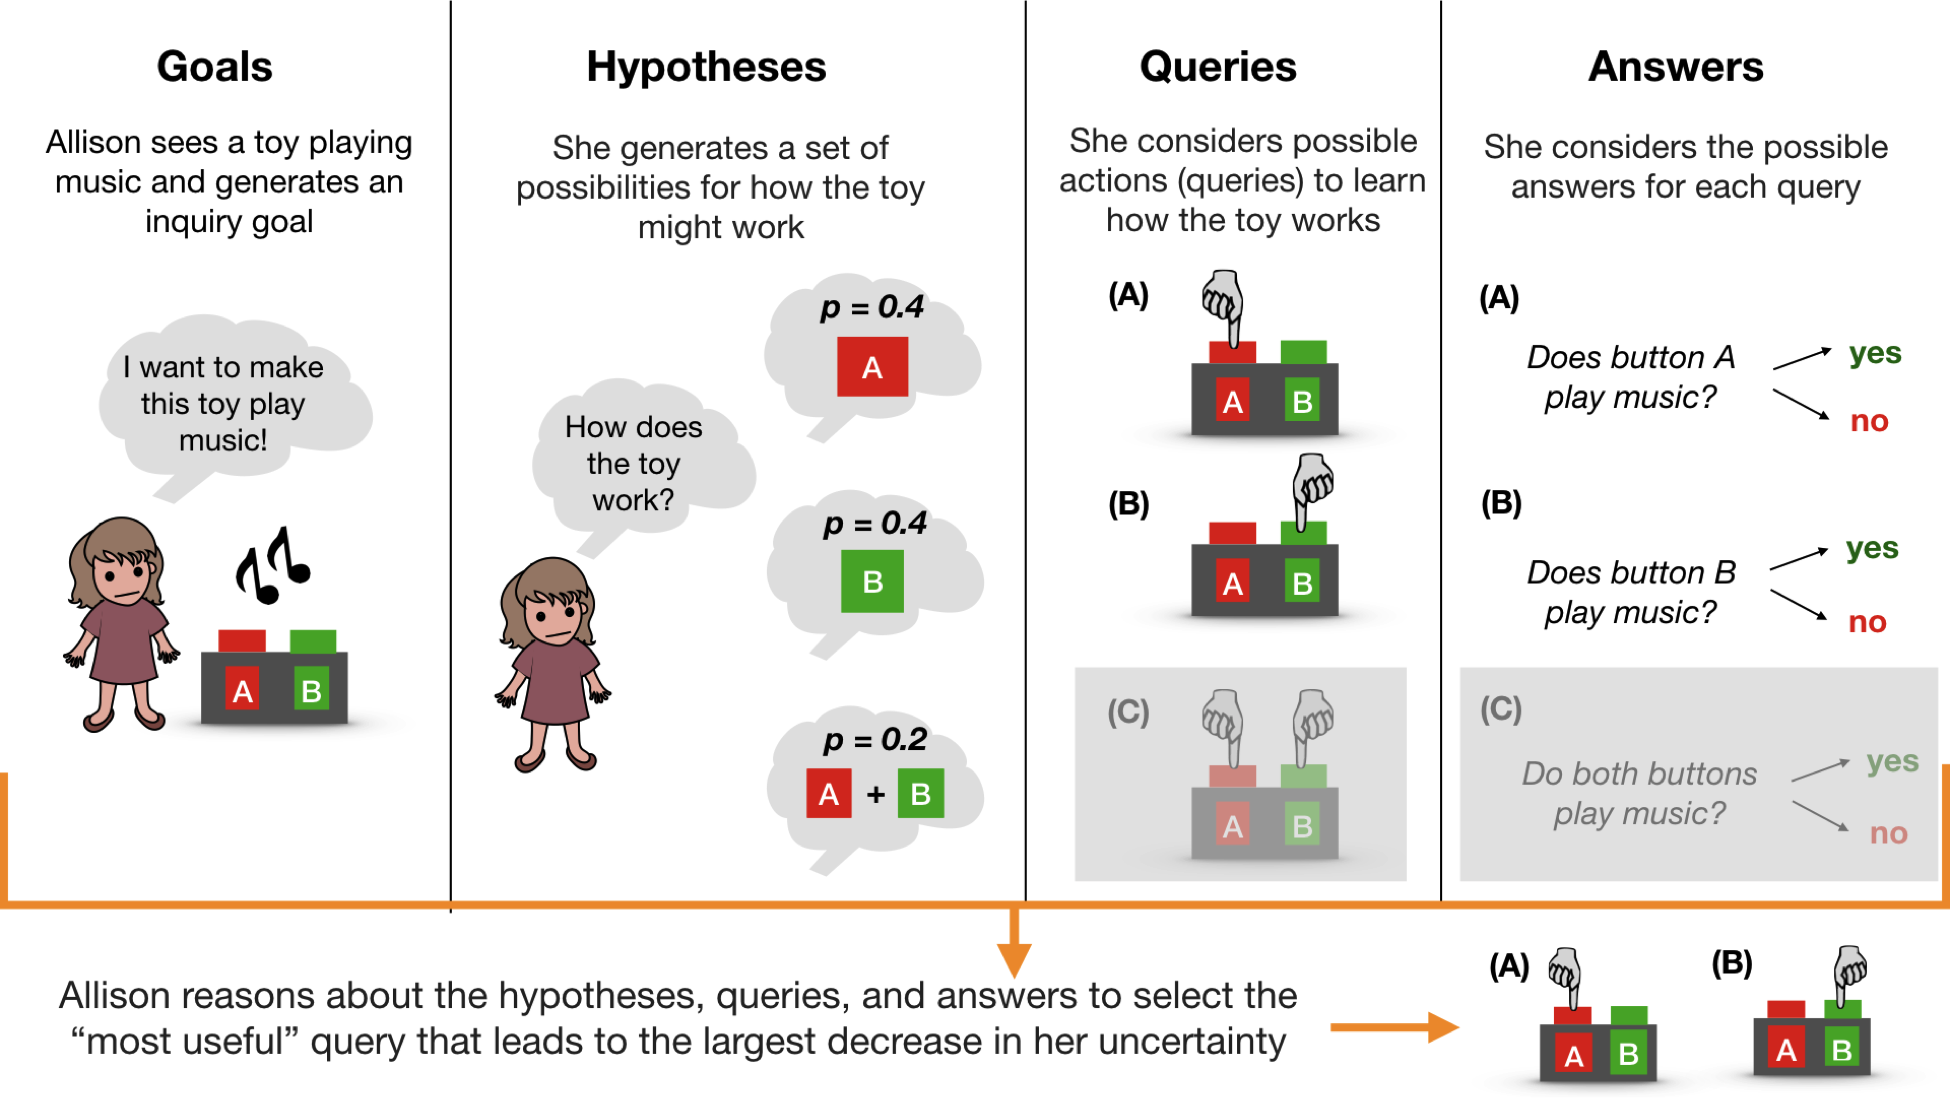
\includegraphics[width=1\linewidth]{macdonald_cada_files/figure-latex/unnamed-chunk-1-1} \caption{Schematic active learning context using the decomposition of Optimal Experiment Design. The learner generates an inquiry goal. Then she considers her hypotheses, possible queries (actions), and the potential outcomes of those actions. Together, these components quantify the expected usefullness of each action, and if the learner chooses optimally, then she picks the action that maximizes this expected utiltiy. See the OED section in the text for the mathmatical details.}\label{fig:unnamed-chunk-1}
\end{figure}

Optimal Experiment Design (OED) (Emery \& Nenarokomov, 1998; Lindley,
1956; Nelson, 2005) is a statisical framework that attempts to quantify
the \enquote{usefulness} of each experiment within the set of possible
experiments that an experimenter could conduct to improve their
understanding of a phenomenon. The key insight was described by Lindley
(1956) as a transition from viewing the practice of statistics as making
binary decisions about what to do next to the practice of gathering
information in order to sharpen one's understanding of the
\enquote{state of nature} (p.~987), More concretely, he proposed that
experiments should be designed to maximize a measure of expected
information gain (derived from Information Theory and discussed in more
detail below) and that researchers should continue the experiment until
some pre-determined threshold of information is reached.

The benefit of using the OED approach is that it allows scientists to
make design choices that maximize the effectiveness of their
experiments, thereby reducing inefficiency and the costs related to
additional experimentation. Consider the following toy example borrowed
from Ouyang, Tessler, Ly, and Goodman (2016) where an experimenter is
interested in designing the best experiment to figure out whether people
think a coin is fair or biased (i.e., a trick coin). Here the
researcher's hypotheses correspond to different models of the coin --
\(M_{fair}: Bern(\frac{1}{2})\) and \(M_{bias}: Bern(p)\) where
\(p \sim Uniform(0,1)\) -- and the experiments correspond to different
sequences of coin flips she could select as stimuli. Imagine the
researcher is constrained by time or resources and can only show a
sequence defined of four coin flips, creating a space of 16 possible
experiments. The OED framework allows the researcher to select the most
inofrmative experiment that maximize her ability to to differentiate
between the two hypotheses. More concretely, it provides an answer to
the question of how much better it would be to conduct the experiment
\(HHHH\) versus \(HTHT\). In this toy scenario, \(HHHH\) is a more
informative experiment because the bias and fair models make the same
predictions for the \(HTHT\) experiment, meaning we learn little about
the hypotheses from this experiment.

An applied example comes from Nelson, McKenzie, Cottrell, and Sejnowski
(2010). They used OED principles to differentiate competing theories of
information seeking during adults' category learning. That is, they
wrote down an OED model of their category learning task (classifying a
set of images into one of two categories), the possible design choices
(e.g., what combination of features to show participants), and the
relevant behavioral hypotheses (i.e., different theories of category
learning). And using the model, they were able to figure out the
stimulus set where the competing theories made different predictions.

A growing body of psychological research has used the OED framework as a
metaphor for human active learning. The idea is that when people make
decisions about how to act on the world, they are engaging in a similar
process of evaluating the \enquote{goodness} of these different actions
(i.e., experiments) relative to some learning goal, and in turn, select
behaviors that maximize the potential for gaining information about the
world. One of the major successes of the OED model is that it can be
used to account for a wide range of information seeking behaviors,
including verbal question asking (Ruggeri \& Lombrozo, 2015), planning
interventions in causal learning tasks (Cook et al., 2011), and
decisions about where to look during scene understanding (Najemnik \&
Geisler, 2005).

Coenen, Nelson, and Gureckis (2017) provide a thorough review of the OED
framework and its links to research on the psychology of human
information seeking. In their review, they lay out the four critical
parts of an OED model: 1) a set of hypotheses, 2) a set of questions
(i.e., actions) to learn about the hypotheses, 3) a way to model the
types of answers that each question could elicit, and 4) a way to score
each of the possible answers with respect to some usefulness metric. In
addition to the components internal to the model, they highlight the
importance of understanding learners' inquiry goals (e.g., \enquote{How
does this toy play music?}) for engaging in OED-like reasoning. The key
point is that without a clear learning goal, then it becomes difficult
to instantiate the hypotheses, questions, and answers that a learner
should consider when deciding what to do next. In the rest of this
section, I provide the mathematical details of the OED approach as
described in Coenen et al. (2017). The goal is to provide structure for
the concpetual analysis of how social learning contexts can intervene on
different components of the OED model.

The goal of an OED model is to formalize the reveleant hypotheses,
queries, and answers such that the learner can quantify the
\emph{expected utility} of different actions she could take. Formally,
the set of queries is defined as \(Q_1, Q_2,..., Q_n = \{Q\}\). And the
expected utility of each query (\(EU(Q)\)) is a function of two factors:
(1) the probability of obtaining a specific answer to a question
\(P(a)\) weighted by (2) the usefulness of that answer for achieving the
learning goal \(U(a)\). Thus, the expected utility for a specific
question \(Q\) is defined as the sum of the utilities for each possible
answer to that question weighted by the probability of getting that
answer (\(P(a)\)).

\[EU(Q) = \sum_{a\in q}{P(a)U(a)}\] \noindent
There are a variety of ways to define the usefulness function to score
each answer. An exhaustive review is beyond the scope of this paper, but
for a detailed analysis of different approaches to modelling the
usefulness of actions with respect to information seeking, see Nelson
(2005). However, one common approach is to use the \emph{information
gain} of an answer, which is defined as the change in the learner's
overall uncertainty before and after receiving the answer. One way to
instanstiate this idea is to compute the change in entropy\footnote{Information
  entropy can be thought of as a measure of unpredictability or the
  amount of uncertainty in the learner's probability distribution over
  hypotheses. Intuitively, higher entropy distributions are more
  uncertain and harder to predict outcomes. For example, if the learner
  believes that all hypotheses are equally likely, then they are in a
  state of high uncertainty/entropy. In contrast, if the learner
  strongly believes in one the hypothses, then her uncertainty/entropy
  is low.} (i.e., uncertainty) after getting a particular answer.

\[P(h|a) = ent(H) - ent(H|a)\]

\noindent
Where the prior entropy \(ent(H)\) can be defined using Shannon entropy
(MacKay, 2003), which provides a measure of the overall amount of
uncertainty in the learner's beliefs about the candidate hypotheses.

\[ent(H) = -\sum_{h\in H}{P(h)log_2P(h)}\] \noindent
The posterior entropy \(ent(H|a)\) is computed the same way but takes
into account how the learner's belief distribution would change after
getting a specific answer.

\[ ent(H|a) = -\sum_{h\in H}{P(h|a)logP(h|a)} \] \noindent
And the likelihood of a hypothesis \(P(h|a)\) can be calculated using
Bayes rule.

\[ P(h|a) = \frac{P(h)P(a|h)}{P(a)}  \]

\noindent

If all pieces of an OED model are defined (hypotheses, questions,
answers, and the usefulness function), then selecting the optimal query
is straightforward. All the learner must do is perform the expected
utility computation for each query in the set of possible queries and
pick the one that maximizes utility. In practice, the learner must
consider each possible answer, score the answer with the usefulness
function, and weight the score using the probability of getting that
answer.

There are several benefits of the OED formalization for understanding
human active learning. First, it forces researchers to define the
different components of an active learning problem, thus making their
assumptions about the phenomenon more explicit. Second, if researchers
are able to develop an OED model, they can ask whether people's behavior
deviates from the optimal behavior predicted by the model. Finally,
casting information seeking as rational \emph{choice} links psychology
with several rich research literatures (economics, statistics, computer
science) that have attempted to formalize decision-making as a process
of utility analysis that includes the costs and benefits of choosing a
particular behavior for information gathering.

One nice demonstration of this approach comes from Nelson (2005) model
of eye movements during novel concept learning. The model combines
Bayesian probabilistic learning, which represents the learner's current
knowledge as a probability distribution over a concept, with an OED
model of the usefulness of a particular eye movement (modeled as a type
of question-asking behavior) for gathering additional information about
the target concept from the visual world. Together, these model
components allowed Nelson (2005) to predict changes in the pattern of
eye movements at different time points in the learning task.
Specifically, they found that early in learning, when the concepts were
unfamiliar, the model predicted a wider, less efficient distribution of
fixations to all candidate features that could be used to categorize the
stimulus. However, after the model learned the target concepts, eye
movement patterns shifted, becoming more efficient and focusing on a
single stimulus dimension.

Recent developmental work has used OED models to test whether children
are capable of selecting efficient behaviors that maximize learning
goals. For example, Legare, Mills, Souza, Plummer, and Yasskin (2013)
used a modified question asking game where 4- to 6-year-old children saw
16 cards with a drawing of an animal on them. The animals varied along
several dimensions, including type, size, and pattern on the animal. The
child's task was to ask the experimenter yes-no questions in order to
figure out which animal card the experimenter had hidden in a special
box. Children's questions were coded as either constraint-seeking
(narrowing the set of possible cards by gathering information about a
particular dimension (e.g., \enquote{Is it red?}), confirmatory
(questions that provided redundant information), or ineffective that did
not provide any useful information (e.g., \enquote{Does it have a
tail?}). All children produced a high proportion of the effective,
constraint-seeking questions and the number of constraint-seeking
questions was correlated with accuracy in guessing the identity of the
card hidden in the special box. Legare et al. (2013) interpret these
results as providing evidence that children can use questions to solve
problems in an efficient manner. Converging evidence in support of this
interpretation comes from experimental work using this approach finding
that children prefer to direct questions to someone who is knowledgeable
compared to someone who is inaccurate or ignorant (Mills, Legare, Bills,
\& Mejias, 2010; Mills, Legare, Grant, \& Landrum, 2011),

Although the OED approach has provided a formal account of seemingly
unconstrained information seeking behaviors, there are several ways in
which it falls short as an explanation of human self-directed learning.
Coenen et al. (2017) argue that OED models make several critical
assumptions about the learner and the learning task, including (1) the
hypotheses/questions/answers under consideration, (2) that people are
actually engaging in some kind of expected utility computation in order
to maximize the goal of knowledge acquisition, and (3) that the learner
has sufficient cognitive capacities to carry out the computations.

In the next section, I argue that limitations of the OED approach can be
productively reconstrued as opportunities for understanding how learning
from other people can scaffold active learning. I focus on integrating
research and theory on social learning with five key components of the
OED model: inquiry goals, hypotheses, questions, answers, and stopping
rules. The key insight is that learning from more knowledgeable others
provides the building blocks for children to engage in effective
self-directed learning.

\begin{figure}[tb]
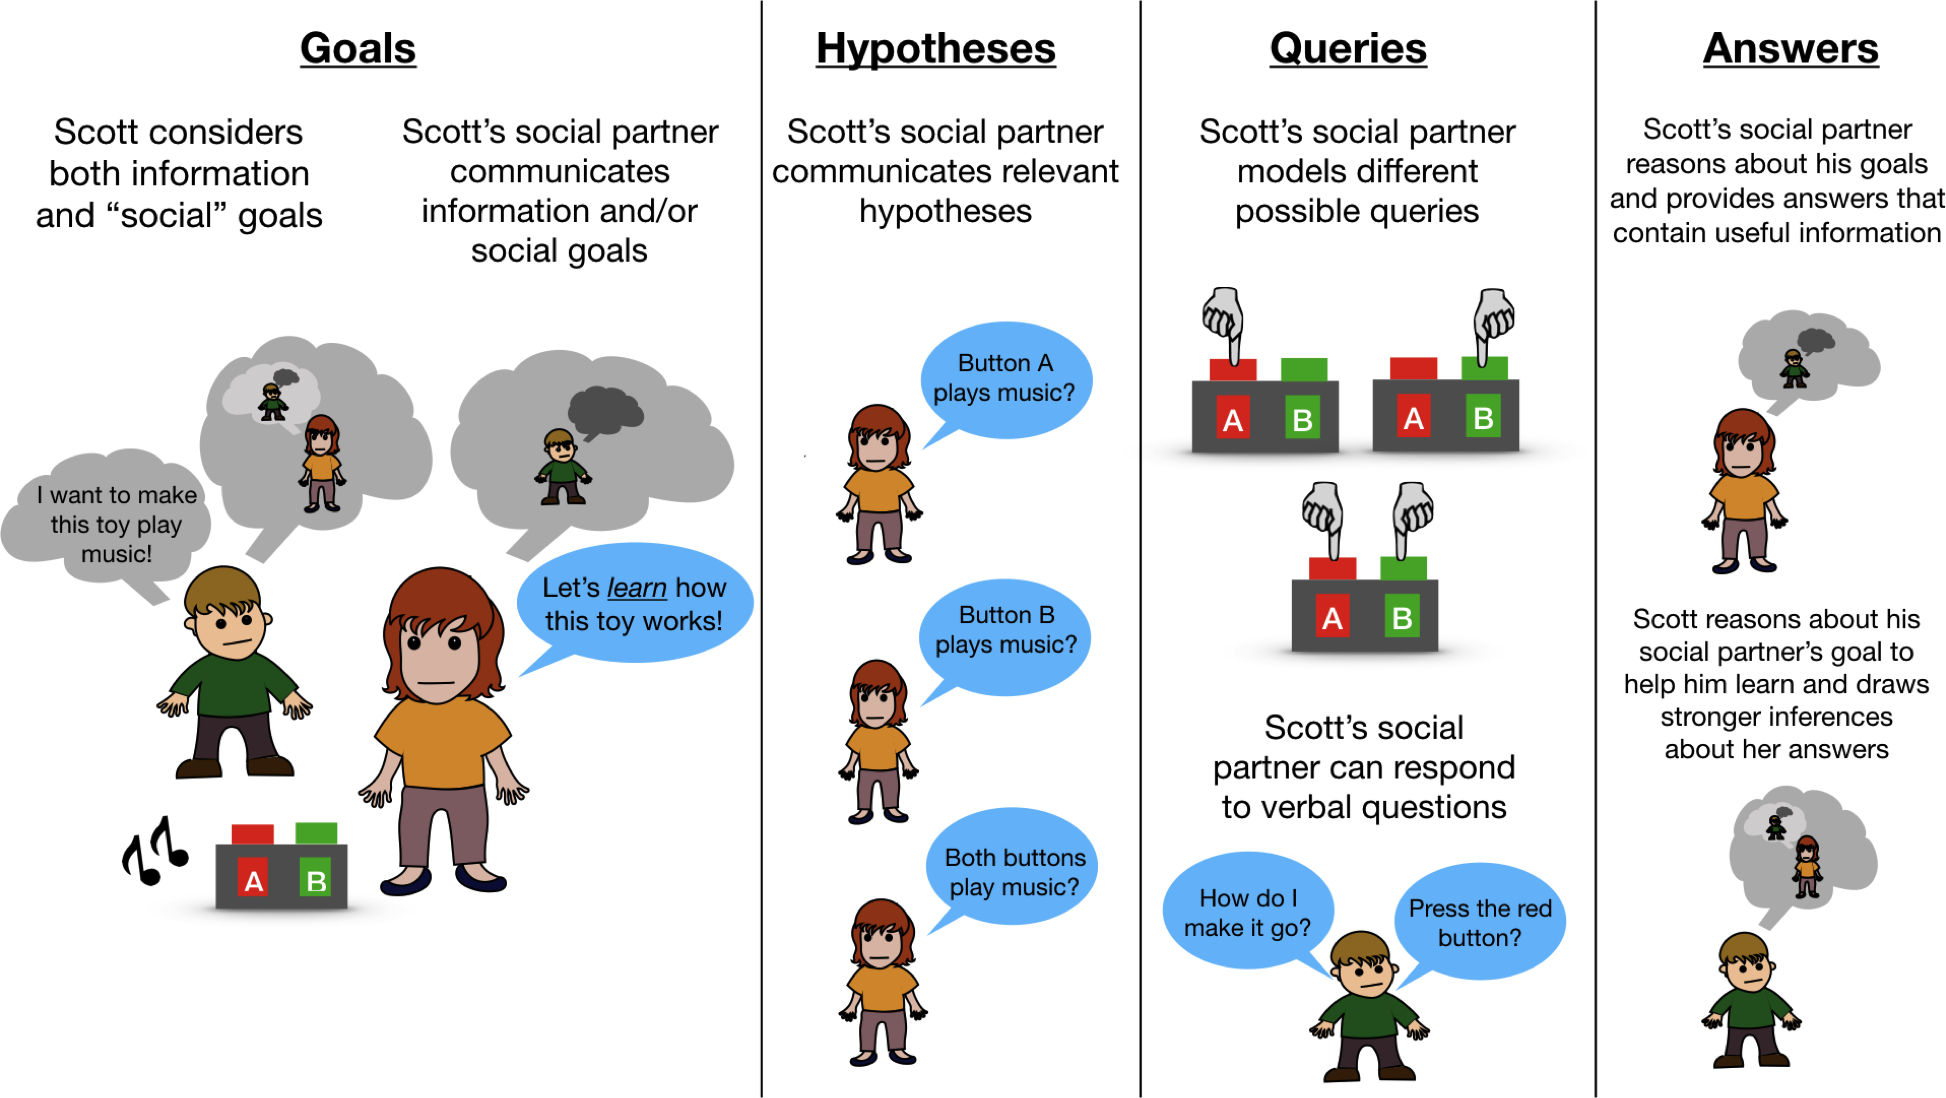
\includegraphics[width=1\linewidth]{macdonald_cada_files/figure-latex/unnamed-chunk-2-1} \caption{Schematic of active learning within a social context.}\label{fig:unnamed-chunk-2}
\end{figure}

\section{Part IV: Active learning within social
contexts}\label{part-iv-active-learning-within-social-contexts}

Why integrate the social and active learning accounts? First, children
do not re-invent knowledge of the world, and while they can learn a
tremendous amount from their own behaviors, much of their generalization
and abstraction is shaped by input from other people. Moreover, social
learning can sometimes be the only way to learn something and sometimes
it can be a faster or more efficient route for learning. Finally,
children are often surrounded by parents, other knowledgeable adults,
and older peers -- all of whom may know more about the world than they
do, creating contexts where the opportunity for social learning is
ubiquitous.

In addition, there is a body of empirical work showing that active
learning can be biased and ineffective in systematic ways. For example,
work by Klahr and Nigam (2004) showed that elementary school-aged
children were less effective at discovering the principles of
well-controlled experiments from their own self-directed learning, but
were capable of learning these principles from direct instruction. D. B.
Markant and Gureckis (2014) showed that active exploration provided no
benefit over passive input in an abstract category learning task when
there was a mismatch between the target concept and adults' prior
hypotheses going into the learning task. And McCormack et al. (2016)
found that 6-7 year-olds showed no learning benefits when allowed to
actively intervene in a causal system compared to observing another
person performing the interventions, which the authors suggest might be
due to the relative decrease in cognitive demands in the observational
learning condition.

In a comprehensive review of the self-directed learning literature,
Gureckis and Markant (2012) point out that the quality of active
exploration is linked to aspects of the learner's understanding of the
task: if the representation is poor, then self-directed learning will be
biased and ineffective. Coenen et al. (2017) go a step further and
outline the challenges of demonstrating efficient active learning
behaviors. Might social learning accounts have something to say in
addressing the mixed results and challenges in the self-directed
learning literature?

This section proposes one potential solution to the challenge of
characterizing children's learning as efficient information seeking
guided by OED principles. I take the OED model outlined in Coenen et al.
(2017) as a starting point for defining efficient inquiry behavior, and
use it to integrate social and active learning accounts. The benefit of
this formal framework of self-directed learning is that it makes the
different components of active learning explicit and highlights aspects
that might be particularly challenging for young learners with limited
cognitive resources.

I propose that we can reconstrue the \enquote{limitations} of the OED
account as a model of human learning as opportunities for understanding
how social contexts (i.e., interactions with more knowledgeable others)
can support information seeking. In each section, I highlight the
developmental challenge for each component of the OED model and then
discuss how features of the social learning context could influence play
a role. I also highlight prior work that highlight the potential for
social contexts to shape self-directed learning and point to
interesting, open questions that are promising areas for future work.

\subsubsection{Goals}\label{goals}

An inquiry goal refers to the underlying motivation for people's
information seeking behaviors. Often this is simply defined as a search
for the correct hypothesis amongst a set of candidate hypotheses.
Intuitively, an inquiry goal is what drives people to learn. Some
examples of plausible inquiry goals that span across a variety of
learning tasks and developmental research literatures include:

\begin{itemize}
\tightlist
\item
  Is this person a reliable source of information? (selective learning)
\item
  What is this speaker referring to? (referential uncertainty)
\item
  What types of objects are called \enquote{daxes}? (category learning)
\item
  How does this toy work? (causal learning)
\item
  Where should I look next? (allocation of visual attention)
\end{itemize}

\noindent
Without an explicit inquiry goal, it becomes difficult for an active
learner to compare the quality of different behaviors since the learner
cannot evaluate how an action will lead to learning progress. Coenen et
al. (2017) illustrate this point by highlighting how researchers often
go to great lengths to communicate the specific inquiry goal of an
experimental task, saying:

\begin{quote}
\enquote{The importance of such goals is made clear by the fact that in
experiments designed to evaluate OED principles, participants are
usually instructed on the goal of a task and are often incentivized by
some monetary reward tied to achieving participants that goal.
Similarly, in developmental studies, children are often explicitly asked
to answer certain questions, solve a particular problem, or choose
between a set of actions.} (p.~32-33)
\end{quote}

\noindent
Thus, characterizing children's goals during learning becomes critical
for evaluating the quality of self-directed learning behaviors. However,
this is no easy task since children could be considering a wide range of
goals during any moment and there is no guarantee that learning progress
should be one of the goals. In fact, one line of theorizing about OED as
a model of human inquiry argues that we should only expect to see
efficient information seeking behaviors in contexts where there is a
clear task and learning goal. For example, when a parent gives their
child a new toy with several buttons on it and the child's goal is to
figure out how to make it work. In this case, we could ask whether the
child approaches the learning task in an efficient way, selecting
actions that are most likely to provide useful information about the
toy's causal structure.

In the previous example, we see the potential for children's
interactions with more knowledable others to play a role in triggering
inquiry behavior. That is, adults and older peers have the capacity to
construct contexts with clear learning goals in order to support
children's own information seeking. This connection draws on influential
ideas in cognitive development that frame social learning as a form of
scaffolding where children are placed in contexts that present something
new to be learned but importantly conatin learning goals that are
achieveable given children's current capabilties (e.g., Zone of Proximal
Development (Vygotsky, 1987), Rogoff's theory of Guided Participation
(Rogoff et al., 1993), and more recently Guided Play (Weisberg,
Hirsh-Pasek, \& Golinkoff, 2013)).

For example, Weisberg et al. (2013) define guided play as an
intermediate learning context that falls between totally unstructured
free play and constrained direct instruction. The boundaries between
these contexts are difficult to define, but the critical dimension is
the level of control that the more knowledgable participant exerts over
the activity. In free play, the child decides what to do next; whereas
in direct instruction, the more knowledgable person explicitly tells the
learner what to do, asks questions, or demonstrates new concepts.

In their review, they present the following example to illustrate the
key difference between guided play and direct ins

\begin{quote}
For example, a teacher with the goal of teaching new vocabulary words
could take a direct instruction approach, by telling children the
meanings of the new words they encounter in a storybook or by showing
examples: \enquote{This is a helmet. A helmet goes on your head to stop
your head from getting hurt if you fall off your bike.} Or, she could
take a guided-play approach, introducing the new words in the context of
a child's play episode while encouraging children to think broadly about
the word's meaning: \enquote{She's got a helmet on while riding her
bike. What do you think would happen if she fell off her bike and wasn't
wearing her helmet?} (p.~106)
\end{quote}

\noindent
While these contexts appear quite similar, the key difference is whether
the child initiated the activity. Weisberg et al. (2013) hypothesize
that guided play context provides the right combination of structure
with the opportuntity for children's to exercise self-efficacy over
learning, and leads to better learning outcomes.

One less-emphasized feature of the Guided Play proposal is the
importance of an adult initializing a clear learning goal for the
activity. In the previous example, if we removed the adult and only
provided the child with a storybook to explore, it is unclear what goals
the child would pursue when deciding what actions to take. However, the
very presence of an adult who has knowledge of the names of objects in
the book and has the goal to teach those names to the child changes the
potential for the child to engage in informations-seeking behaviors.
More formally, we can connect this example to the OED framework of
self-directed learning, and it becomes clear that one potentially
important role of more knowledable others is to present children with a
clear learning goal, which in turn sets the stage for children to reason
about what actions to take next (e.g., what question to ask or what
object to point at) and how those actions might best support the current
learning goal (i.e., learning the names of objects in the storybook).

Another interesting connection between social contexts and children's
inquiry goals comes from a body of work exploring how children's input
shapes their implicit theories of intelligence and in turn influences
the goals they choose to pursuse in novel learning contexts (Dweck \&
Leggett, 1988). Specifically, implicit theories of intelligence refer to
children's internal working models of the world and provide general
frameworks for processing information and generating predictions about
behavior. Dweck and Leggett (1988) propose a causal model where implicit
theories of intelligence cause different goal orientations, which
interact with perceptions of present ability to generate different
behaviors. For example, if children hold a belief that intelligence is
malleable (an incremental theory), they will want to increase competence
(select a learning goal) and therefore be more likely to select tasks
that support learning (mastery-oriented).

Empirical work has shown that children can be oriented toward learning
goals by an experimenter. For example, Elliott and Dweck (1988) directly
manipulated elementary school-aged children's goals by presenting them
with a choice between one of two tasks described in the following ways:

\begin{itemize}
\tightlist
\item
  Performance task. In this box we have problems of different levels.
  Some are hard, some are easier. If you pick this box, although you
  won't learn new things, it will really show me what kids can do.
\item
  Learning task. If you pick the task in this box, you'll probably learn
  a lot of new things. But you'll probably make a bunch of mistakes, get
  a little confused, maybe feel a little dumb at times --- but
  eventually you'll learn some useful things.
\end{itemize}

\noindent
Elliott and Dweck (1988) found that when children were oriented towards
the learning goal, they tended to choose the more difficult
\enquote{learning} task even though they were likely to make mistakes
and risk looking incompetent. In another study, Dweck and Leggett (1988)
showed that children who already held performance goals viewed effort on
a task as an index of ability, whereas children with learning goals view
effort as a means for improvement. Morever, both lab-based experiments
and observational work provide evidence that the language adults choose
to use when praising chidren can shape how likely children are to hold
implicit theories that emphasize learning over and above performance
goals (Cimpian, Arce, Markman, \& Dweck, 2007; Gunderson et al., 2013).

Taken together, the research on implicit theories suggests another
pathway through which social contexts can trigger inquiry goals. We can
recast the Elliott and Dweck (1988) finding -- that children oriented
toward learning goals select harder tasks -- in terms of the OED
framwork. That is, the goal manipulation is an instance of the social
context initializing an inquiry goal, which in turn influences
children's decision making, leading children to select behaviors that
result in a higher chance of learning new concepts, an explicit
prediction that falls out of the OED model of human inquiry.

Another interesting place where the social context of learning can
impact information seeking is by introducing a set of \enquote{social}
goals that directly impact information seeking behaviors. The basic OED
framework only includes the goal of information seeking, meaning that
the utility of an outcome is based solely on how answers change
probabilities of hypotheses. However, other work has expanded on this
basic information-seeking account to include \emph{situation-specific
utility functions} that allow for other goals such as saving time,
money, or cognitive resources. For example, Meder and Nelson (2012)
designed a series of experiments where \enquote{pure} information
seeking goals (e.g., maximizing accuracy) were placed at odds with the
reward structure of the task. To accomplish this, they used assymetric
rewards for correct and incorrect categorization decisions in a binary
classification task. Asymmetric rewards leads to a scenario where the
learner must choose the less likely category in order to earn the
highest reward (i.e., they must be willing to forego the goal of being
accurate and make mistakes). When task-specific rewards were put in
conflict with accuracy, participants' behavior was mixed -- only when
the asymmetric reward structure was made explicit via language did
participants seek inforation about the higher reward, but lower
information gain feature. Meder and Nelson (2012) speculate that
participants were not only considering information gain or pure reward
maximization goals and take the results as evidence for the need to
consider additional components in the utility function.

One powerful feature of adding a social partner to a learning context is
that it can engage a process of psychological reasoning about their
mental life (e.g., beliefs and goals). Once the learner starts reasoning
about the other person, they could start to consider an additional set
of \enquote{social} goals that may conflict or support their information
seeking goals. For example, if Scott is worried about whether his
teacher thinks he is smart, then he might prioritize actions that
maximize the probability of success in order to demonstrate his
intelligence, perhaps at the expense of choosing actions that maximize
his inquiry goal of learning how to make the toy play music.

Recent work by E. J. Yoon, Tessler, and Frank (2017) has modeled polite
speech (e.g., people using indirect language: \enquote{I don't think
that dress looks phenomenal on you} as opposed to \enquote{It looks
terrible}) as a process of trading off between information and social
goals. Specifically, speakers reason about their actions with respect to
the information goal -- communicate information faithfully and with as
little effor as possible -- and a social goal -- avoid damage to your
own or another person's self-image. To formalize this intuition, E. J.
Yoon et al. (2017) build on the Rational Speech Act framework for
pragmatic reasoning (Goodman \& Frank, 2016), which models language
comprehension and production as, \enquote{\ldots{} a process of
recursive reasoning about what speakers would have said, given a set of
communicative goals} (p.819). The polite RSA model connects with the OED
information seeking model in that both assume that people will produce
an action (in RSA an utterance and in OED a query) to maximize utility,
but the polite RSA expands the speaker's utility function, modeling
overall utility of an utterance as a weighted combination of social and
informational utility.

It would be interesting to modify utility-theoretic approach used by E.
J. Yoon et al. (2017) to children's information seeking behaviors in
social contexts. We can also connect these ideas to the effects of task
framing (peformance vs.~learning oriented) on children's decisions to
try harder tasks. It could be that the presence of another person
increases the weight children place on maximizing social utility,
leading children to select easier tasks where they can appear competent.
This is a subtle but interesting extension of the goal-orienting account
reviewed above in that it frames these effects as a mixture of goals as
opposed to the social context triggering either an performance or a
learning goal.

One important gap in the literature on inquiry goals is a good estimate
of how often children participate in contexts with clear learning goals
in their daily lives, as opposed to contexts where learning goals are
absent or contexts where children are clearly pursuing other
non-learning related goals (e.g., some example here). Moreover, there is
a need for more research on the kinds of events that lead children to
generate inquiry goals. However, Rogoff et al. (1993)'s work on
\emph{Guided participation} provides an interesting counter-example
where they coded the rate of \enquote{caregiver orienting} behaviors in
parent-child interactions with their 12- to 24-month-old infants across
four different cultural communities (a Mayan Indian town in Guatemala, a
middle-class urban group in the United States, a tribal village in
India, and a middle-class urban neighborhood in Turkey) that varied
along the dimensions of how separated children were from adult
activities and whether formal schooling was emphasized. Specifically,
caregiver orienting was defined as doing the following behavior during
parent-child interaction around a set of novel toys,

\begin{quote}
Caregiver orients child involved introducing new information or
structure to the child (at any point in the episode) regarding the
overall goals or a key part of the event or what was expected in the
situation. Orienting framed a major goal, not just specific little
directives for particular actions.
\end{quote}

\noindent
Rogoff et al. (1993) found that parents in all four communities produced
high rates of structuring and orienting behaviors (with the lowest rate
of structuring being 81\% of play episodes). Thus, when placed in a
structured activity, adults make sure children are aware of the goal
(e.g., learning the function of the novel toy). However, the communities
differed in how often children were directly involved with adult
activities in day-to-day life, with the children raised in rural
villages often having early acces to adult economic and social
activities. An interesting open question is whether older peers and
adults need to be directly engaging with the child in order to trigger
inquiry goals and efficient self-directed learning behaviors. Perhaps
increased access to observing lots of adult goal-directed behaviors can
faciliate children to generate leanring goals, for example as they see
activies being completed that they do not understand.

One important direction for future research to map the space of
children's goals during everyday learning contexts. It would be
interesting to know the proportion of children's daily activities that
involve contexts where there is a clear learning goal either being
demonstrated by the child or by older peers and adults. It would also be
useful to know how the distribution of these tasks changes as a fnction
of development, especially as children enter school and across different
cultural contexts where children have differential access to structured
(e.g., lessons and sports) vs.~unstructured activies (e.g., free play).

\subsubsection{Hypotheses}\label{hypotheses}

After establishing that there is something to be learned, the next key
component of inquiry is deciding what hypotheses should be considered
and tested. Intuitively, a hypothesis is a candidate explanation about
how the world works. For example, if a child is in a concrete word
learning context -- i.e., she hears a new word (\enquote{dax}) and is
surrounded by a three unfamiliar objects (A, B, and C) -- then she might
entertain at least\footnote{This hypothesis space only considers
  one-to-one mappings.} the following hypotheses about the meaning of
dax: dax = A, dax = B, or dax = C.

The set of hypotheses under consideration is critical for measuring
effective self-directed learning. The usefulness function outlined in
Part II works by comparing the learner's uncertainty over hypotheses
before and after the she performs some action on the world. Without
knowing what is in the hypothesis space, it becomes challenging to
figure out the best action for reducing uncertainty. Put another way,
the OED framework does not easily deal with situations where learners
might have to consider a large space of hypotheses, might actually hold
the wrong hypotheses, or perform actions without considering any
hypotheses at all. This scenarios seem plausible for young learners and
thus present a challenge to using OED principles as a model of early
active leanring.

However, one important functions of social learning contexts is to
provide a clear set of possible explanations for the true state of the
world. That is, adults and older peers, who might have access to the
correct hypothesis, can restrict the hypothesis space in order to help
guide children information seeking behaviors. The effect of social
contexts on hypotheses parallels the effect on goals reviewed in the
previous section: that the behaviors of other people have the capacity
to initialize and constrain.

One relevant case study of the capacity for social contexts to constrain
hypotheses comes from work on children's early word learning. The
challenge for the young word learner is that even the simplest of words,
concrete nouns, are often used in complex contexts with multiple
possible referents, which in turn have many conceptually natural
properties that a speaker could talk about. This creates the potential
for an (in principle) unlimited amount of hypotheses that children could
consider for the meaning a novel word. Remarkably, word learning
proceeds despite this massive uncertainty, with estimates of adult
vocabularies ranging between 50,000 to 100,000 distinct words (P. Bloom,
2002).

It does not seem plausible for children to entertain all hypotheses
about possible word-object links. But how might children constrain the
hypotheses that they consider? One proposed solution is for word
learners to only consider a single word-object hypothesis at a time
(Medina, Snedeker, Trueswell, \& Gleitman, 2011; Trueswell, Medina,
Hafri, \& Gleitman, 2013). That is, the child could make an initial
guess about the meaning of a new word, and then only consider that guess
until she receives sufficient evidence that her initial hypothesis was
incorrect. If she seees sufficient counter-evidence, then she will
switch to a new hypothesis that better matches the statistics in the
input.\footnote{This \enquote{propose-but-verify} account parallels work
  by E. Bonawitz, Denison, Gopnik, and Griffiths (2014) in the domain of
  causal learning, which suggests that a \enquote{Win-Stay, Lose-Sample}
  algorithm (inspired by efficient sampling procedures in computer
  science) provides a better explanation of children's hypothesis
  testing behaviors compared to an algorithm that enumerates the entire
  hypothesis space.} Another influential account of early word learning,
inspired by basic associative learning principles, argues that children
store more than a single hypothesis, suggesting that the hypothesis
space is gradually reduced via the aggregation of word-object labels
across multiple labeling events (Siskind, 1996; C. Yu \& Smith, 2012b).
Support for this experimental work has shown that both adults and young
infants can use word-object co-occurrence statistics to learn word
meaning from individually ambiguous naming events (Smith \& Yu, 2008).
Moreover, adults show evidence of being able to recall multiple
word-object links from an initial naming event (Yurovsky \& Frank,
2015).

The key difference between these proposals is how much information
learners store in their hypothesis space. Understading the nature of the
hypotheses that learners consider is critical for evaluating children's
ability to seek information with respect to those hypotheses. Some of
our own work provides direct evidence that the social context of
language learning can modulate the content of the learner's hypothesis
space (MacDonald, Yurovsky, \& Frank, 2017). Inspired by ideas from
Social-pragmatic theories of language acquisition that emphasize the
importance of social cues for word learning (P. Bloom, 2002; Clark,
2009; Hollich et al., 2000), we showed adults a series of word learning
contexts that varied in ambiguity depending on whether there was a
useful social cue to reference (i.e., a gaze cue). We then measured
learners' memory for alternative word-object links at different levels
of attention and memory demands. Results showed that learners flexibly
responded to the amount of ambiguity in the input, and as uncertainty
increased, learners tended to store more word-object links. Morever, we
found that learners stored representations with different levels of
fidelity as a function of the reliability of the social cue and despite
having the same amount of time to visually explore the objects during
the initial labeling event.

These results suggest that the content of learners' hypothesis spaces
changed as a function of the quality of the social learning context.
Further suppport for this idea comes from experimental work showing that
even children as young as 16 months prefer to map novel words to objects
that are the target of a speaker's gaze and not their own (D. A.
Baldwin, 1993), and analyses of naturalistic parent-child labeling
events shows that young learners tended to retain labels that were
accompanied by clear referential cues, which served to make a single
object dominant in the visual field (C. Yu \& Smith, 2012a). One
important direction for future research is to measure the full causal
pathway from variation in social learning contexts to the nature of
children's hypothesis spaces and their information seeking behaviors.
For example, it would be interesting to know whether learners'
subsequent information seeking behaviors would be affected by social
context manipulations like the ones used in our task.

A second case study that illustrates the importance of considering young
learner's hypothesis spaces comes from work by Lucas, Bridgers,
Griffiths, and Gopnik (2014) where they compared chidren and adult's
capacity for learning different kinds of causal structures. In the task,
participants were shown a series of events that consisted of a training
phase where an experimenter placed objects on a box that either did not
did not play music. The participant's goal was to learn which objects,
or combination of objects, made the box work. In the disjunctive
condition, only single objects (A or C, but not A) made the toy play
music. In the conjunctive condition, only the combination of two
different objects (A and C) would make the toy play music. After seeing
several demonstrations, both children and adults were tested on
ambiguous events where they could either infer a disjunctive or
conjunctive causal relationship. Lucas et al. (2014) found that only
children showed evidence of learning the conjunctive relationship, even
if the evidence favored this interpretation. The authors speculate that
children have less of a bias towards preferring the disjunctive
relationship, which is more common in everyday experience, and are thus
better able to learn from new evidence.

Why might these findings matter for active learning? A key prediction of
the OED account is that learners will select behaviors that maximally
reduce uncertainty in their beliefs, which is often formalized as the
difference in entropy between the prior and posterior probability
distributions over hypotheses (i.e., \(P(h|a) = ent(H) - ent(H|a)\)).
Thus, the content of the hypothesis space and the uncertainty over each
hypothesis plays a direct role in evaluating the relative usefulness of
different information seeking behaviors. Moreover, the social context
could play a role in setting up the hypothesis space. For example, Lucas
et al. (2014) suggest that,

\begin{quote}
Most of the time, adults do not need to dramatically change their
beliefs or abandon their hypotheses for dramatically different ones.
Indeed, doing so would be a liability: adults are expected to make
accurate predictions and good decisions, not bold inductive leaps.
Adults are also unlikely to have caregivers to correct their errors and
save them from poor choices.
\end{quote}

\noindent
This makes an interesting, testable prediction that contexts where
learners \enquote{feel} safe to make mistakes would lead children to
consider and test a broader range of hypotheses. Moreover, another
effect of the social context is highlighted in Lucas et al. (2014)'s
study: that the experimenters went to great lengths to ensure that
children and adults would only consider the disjunctive and conjunctive
hypotheses. That is, they constrained the hypothesis space to isolate
learning and information seeking effects. It is an interesting and open
question as to how often this type of process occurs in everyday
learning contexts.

A final case study demonstrating the link between social input and
children's hypotheses comes from research on conceptual change (Gelman,
2009). Conceptual change refers to a \enquote{radical} reconstruction of
an intuitive theory about how the world works based on some intervening
factor. For example, elementary school-aged children tend to hold a
mixture of beliefs about the shape of the earth (Vosniadou \& Brewer,
1992). These theories range from flat earth theories that match
children's everyday perceptual experiences (i.e., walking on flat
ground) to the adult-like, sphere model, which must have been learned
via social input. Intrestingly, children also show evidence of holding
interemtidate beliefs such as a dual-earth theory where there are two
earths, \enquote{a round one which is up in the sky and a flat one where
people live} (p.~550). The fact that children entertain something like
the dual-earth theory suggests that they are actively trying to
integrate their initial theory with information they get from
interactions with people who already have the correct, sphere theory.

There is also strong experimental evidence for the importance of social
input in children's theory revision. For example, in the domain of
biological reasoning, the concept of \enquote{alive} takes years to
fully develop, with younger children (under 10 years of age) often
claiming that only animals, and not plants, are alive. Opfer and Siegler
(2004) tested the hypothesis that evidence of goal-directed movement is
critical for children's extension of the \enquote{alive} concept. In
their study, 5-year-olds' were trained on different ways to think about
the concept of a \enquote{living thing} and then asked whether they
believed that plants were alive. Children either learned that plants
were capable of goal-directed movement (e.g., \enquote{The house plant
is growing this way. It needs the sunlight over here.}), that plants
were capable of growth, or that plants need water to survive. Children
in the goal-directed movement condition showed the strongest evidence
theory revision, saying plants were also living things more consistently
on a post-intervention categorization task.

Additional evidence for the role of social input on children's
hypotheses comes from research on the links between language experience
and performance on various cognitive tasks. For example, empirical work
has shown that deaf children without access to a natural language
perform worse on Theory of Mind tasks (Peterson \& Siegal, 2000), that
Korean speakers perform better than English speakers on tasks that
require categorizing based on tight vs.~loose distinctions, which are
lexicalized in Korean (McDonough, Choi, \& Mandler, 2003), and that
exposure to a first language reduces infants' capacity to detect
non-native phonetic contrasts (Maurer \& Werker, 2014).

Taken together, the findings reviewed in this section illustate several
important points for the active-social learning acount. First, the set
of hypotheses that children consider are likely to be quite different
from adults (and different from what the experimenter thinks the child
is considering). Second, children generate hypotheses using a mix of
prior knowledge, expectations about the current task, and social input.
Critical to this point is that there are (at least) two timescales
through which social learning can shape hypotheses. (1) An in-the-moment
timescale where other people's behavior can constrain the hypotheses
that children consider for the current task -- for example, referential
gaze indicating candidate word-object mappings, or an adult suggesting a
disjunctive (one-block) vs.~a cojunctive (two-block) theory for how to
make a toy work. (2) A developmental timescale where prior interactions
with other people and cultural learning modifies the hypotheses that
children bring to a particular learning task (e.g., the conceptual
change and language effects reviewed above).\footnote{We could make a
  further distinction between the developmental and the cultural
  timescales, where developmental refers to information acquired from
  interactions with others in the child's lifetime (e.g., disjunctive
  causal structures are more likely to occur in the world) and cultural
  refers to information that has accumulated throughout human
  evoluationary history (e.g., access to natural language or concepts
  such as the spherecial earth.)}

TODO: paragraph about open questions for hypotheses.

\subsubsection{Questions}\label{questions}

Questions in the OED framework refer to the experiments that a scientist
can conduct in order to gather information with respect to their
hypotheses about the world. When we consider \enquote{questions} in
human informaion seeking, it's important to note that
\enquote{questions} can map onto a range of information seeking
behaviors, such as verbal questions, pushing a button to figure out how
a toy works, and decisions about where to look. In fact, the capacity to
provide general principles to explain such a broad range of behaviors is
one of the strengths of the OED account as a model of human active
learning.

The challenge for the young learner is to discover what behaviors are
available and of those behaviors which might be particularly good for
gathering information to support learning. In this section, I illustrate
how the social learning context provides the input to this learning
process via demonstrations of the range of actions that learners could
take and by adults' modeling effective information seeking behaviors.

It seems obvious that children would look to older peers or adults to
learn what actions are possible and useful. However, a large body of
empirical work suggests that even young infants will not imitate every
action that they see. Instead, children show evidence of
\enquote{rational imitation} and look for cues about other people's
goal-directed behaviors and use this information to determine what
behaviors are worth imitating . For example, Gergely, Bekkering, and
Király (2002) measured how often 14-month-old infants imitated an
adult's inefficient action -- turning on a light with her head (less
efficient) instead of her hands (more efficient) -- as a function of
whether there was a relevant explanation for selecting the less
efficient action (whether the adult's hands were occupied). They found a
large difference in imitation rates across conditions (69\% in the
hands-free vs.~21\% in the hands-occupied), suggesting that children
recognized the reason for the inefficient action and chose to ignore the
means and focus on the goal of turning on the light in the most
efficient way possible.

The high rates of imitation in the hands-free condition highlight
another important compoenent of learning from others' actions: that
children tend to overimitate behaviors even when these actions are not
directly relevant to the task. For example, Call et al. (2005) compared
imitation behaviors of 2-year-old children after they watched someone
demonstrate how to open a tube using only the necessary actions or using
the actions and a style component that was unrelated to opening the tube
(e.g., removing the tube's cap with an exaggerated twisting motion).
Children imitated the causally irrelevant action at a high rate (93\% of
children), providing evidence that they were focused on reproducing each
of the experimenter's actions and not just reproducing the outcome of
opening the tube.

Other empirical work provides insight into the importance of considering
the social factors that influence whether children choose to imitate.
Carpenter, Akhtar, and Tomasello (1998) showed that 14- and
18-month-olds were less likely to imitate adults' action if the action
was accompanied by a verbal cue that flagged the action as a mistake
(e.g., \enquote{Whoops!}). Buchsbaum, Gopnik, Griffiths, and Shafto
(2011) provide evidence that the children are more likely to overimitate
when the adult is described as a \enquote{knowledgeable} teacher as
oppossed to \enquote{naive.} And Carpenter, Call, and Tomasello (2002)
showed that giving children explicit information about another person's
goals prior to a causal demonstration leads to an increase in imitation
and learning of the correct casual structure.

Taken together, the work on children's learning via imitiation and their
tendency to overimitate suggests that inferences about others'
intentions plays a critical role in the actions that children will use
in their own behaviors. For the purpose of this paper, this work
provides a way forward for understanding the origin of the information
seeking behaviors that might be available to children, i.e., what are
the available actions that a learner could take to gather information.

One domain where progress has been made in understanding how social
contexts directly shape children's information seeking capacities is
verbal question asking. Consider that in order to ask a useful question
in natural language, children must possess the requisite language
skills, which are learned from their language input. Both experimental
work and corpus analyses provide evidence that children's
question-asking becomes more varied and effective over the first years
of life (e.g., see Chouinard et al. (2007) and Legare et al. (2013)
reviewed in Part II). Moreover, children improve in the timing of their
turn-taking during question-answer exchanges, reducing the length of
gaps between turns (Casillas, 2014). Interestingly, Casillas (2014) also
found that adults appeared to be sensitive to children's developing
question-answering skills by asking more difficult questions (i.e.,
questions that required more complex answers) as children to older
children and by modifying questions that appeared to confuse children
(e.g., \enquote{Who is this? What's he called? Who is he? What is his
name?}). It is interesting to consider how children might internalize
these modifications as part of their own question asking behaviors.

The majority of the work on children's question asking has focused on
aspects of the child's behavior, exploring how the type, content, and
effectiveness of questions changes as children develop. However, several
studies have measured aspects of caregivers question asking. For
example, B. Yu Yue (2017) coded parent-child interactions from the
CHILDES database to measure the amount of \enquote{pedagogical}
questions in children's input. They differentiate \enquote{information
seeking} questions from \enquote{pedagogical} questions, by coding
whether the adult already knew the answer (e.g., \enquote{What's that
called?}\enquote{;}What does this button do?" vs. \enquote{What did you
do at school?}), and interpreted the goal of the pedagogical questions
as helping the child learn. Results showed that approximately 30\% of
parents' questions were pedagogical, 60\% were information seeking, and
10\% were rhetorical (i.e., not intended to be answered verbally).
Parents also directed a smaller proportion of pedagogical questions to
older children.

More experimental work linking adults' question-asking practices to
children's behaviors is needed. This is especially interesing since
observational studies have found that that parents' use of wh-questions
predicts children's later vocabulary and verbal reasoning outcomes
(Rowe, Leech, \& Cabrera, 2017) and children of parents who were trained
to ask \enquote{good} questions during bookreading episodes at home also
asked better questions during bookreading sessions at school (Birbili \&
Karagiorgou, 2009). One explanation for these associations is that
wh-questions challenge children to produce more complex verbal responses
that in turn builds verbal abilities. However, another interesting
possibilty is that the frequency and type of questions that parents ask
serve as models that could shape children's information seeking
abilities by providing templates for useful behaviors.

Generating a set of questions represents the first step in efficient
information seeking. Next, children have to evaluate the relative
\enquote{goodness} (i.e., utility) of different behaviors. But how do
children learn the features of a good question? One solution is to
observe other people's question asking, recognize which questions are
useful, and imitate those behaviors.

In fact, there is evidence from work with adults that shows a large
difference between people's question-generating (harder) and
question-evaluation (easier) skills. For example, Rothe, Lake, and
Gureckis (2015) asked a group of adults to play a modified version of
the game \enquote{Battleship} where they had to find the location of
three ships that considted of 2-4 tiles and could oriented in either the
vertical or horizontal direction on a 6x6 grid. Participants gathering
information sequentially by uncovering one tile at a time. At different
points in the task, the game would stop and participants were given the
opportunity to ask any question using natural language. Rothe et al.
(2015) used a formal model of the expected information gain of each
question (i.e., the expected reduction in uncertainty after getting the
answer) to evaluate the quality of adults' free-form questions. Results
showed that people rarely produced high information value questions.
However, in a follow-up experiment Rothe et al. (2015) had a different
group of adults play the same game, but this time they provided the list
of questions generated by participantsin the free-form version, and in
this contexts, adults were quite good at selecting high information
value questions.

Developmental work provides evidence of the same generation-recognition
asymmetry. First, experimental work has shown that children younger than
the age of three have difficulty generating appropriate verbal questions
compared to their older peers in \enquote{Twenty Questions} task
designed to measure question-asking skill (Mills et al., 2010, 2011).
However, when Mills, Danovitch, Grant, and Elashi (2012) tested 3- to
5-year-old's capacity to learn from observing third-party
question-answer exchanges. They found that even the youngest children
were capable of using information elicited by others' yes/no questions
to identify the contents of a box. Interestingly, children
differentiated the usefulness of others' question-answer exchanges,
paying more attention to them as compared to exchanges of irrelevant
information.

Together, these results suggest that even at an age where generating
questions \enquote{from scratch} might be difficult, children can
observe and learn from questions that occur in their social environment.
Mills et al. (2011) also explored this phenomenon by directly
manipulating whether children were exposed to a training phase where
adults modeled effective questions prior to playing the question asking
game. They found that even though children were not successful at
constructing good questions on their own, they were able to ask
effective questions at much higher rate following explicit modeling.

Work with elementary-school-aged children in the domain of scientific
inquiry also shows that generating a good question is a challenging
aspect of inquiry skills. One particular relevant example come from Kuhn
and Pease (2008)'s 3-year intervention study that compared children who
were directly trained on inquiry skills (e.g., understanding the
objectives of inquiry and identifying questions) to a group of slightly
older students who had not participated in the training. Children in the
training group showed progress in the skills, but children in the
comparison group failed to develop these skills in the absence of the
particular kinds of input. Summarizing one of the key results,
\textgreater{} Consistent with the findings of Kuhn and Dean (2005),
identifying a question appears to play a key role in making the rest of
the inquiry cycle productive. In the probabilistic version of Ocean
Voyage in year 2, for example, students floundered until they were
helped to formulate a specific research question. Like other components
of the inquiry process, this skill is not one a student learns once and
has mastered.

\noindent
A final example of how social contexts change the set of possible
questions is the very fact of having other people around adds a social
\enquote{target} for information seeking behaviors. This is in contrast
to the effects of social context discussed until this point that serve
as inputs that shape subsequent information seeking behaviors.
Intuitively, if a child is trying to learn how a toy works, they could
try actions to test the system directly (i.e., seek information directly
from the world). But if another perosn is present, then they can choose
to ask questions or seek help via noverbal means (i.e., seek information
directly from another person). Thus, the very presence of another person
modifies the choices that are available to the learner.

Recent empirical work has begun to explore the factors that affect
children's decisions about whether to seek information from the world or
from other people. For example, Fitneva, Lam, and Dunfield (2013) had 4-
to 6-year-old children decide how toto learn about a novel social
category: \enquote{moozles.} The concept was either visible (e.g., the
color of hair) or invisible (e.g., an internal preference). Children
were given a choice of looking directly at the moozle or asking a moozle
expert. Six-year-olds chose to look for a visible property and to ask
for an invisible property above chance in both experiments; whereas
four-year-olds behavior was a bit noisier but showed a preference for
the rational looking behavior with additional cueing in a follow-up
experiment.

Other relevant examples comes from work on children's help-seeking
behavior. Vredenburgh and Kushnir (2016) had children build toys that
required multiple steps, and on each each step children were given the
opportunity to ask for help from the experimenter. Each step varied in
difficulty and children naturally varied in their toy building skill.
Children asked for help when the step was harder, and less competent
children asked for help more often, suggesting that preschoolers sought
help in a systematic way -- when they needed it and not when they
didn't. Moreover, work by Gweon and Schulz (2011) found that
16-month-old infants are selective in help-seeking, turning to a social
target to seek information or acting directly on the world depending on
which information source ws more likely to help them reach their current
goal. In this case, the infants' goal was to make a malfunctioning toy
produce music and the critical manipulation was whether children saw
evidence that explained the likely cause of failure being the toy versus
their capacity for making the toy play music. When the toy was likely to
be broken, they reached for a new object (queried the world), but in
contrast, when the evidence suggested that the child was the issue, then
they sought help from a nearby adult.

Some of our own work has explored how the presence of another person
might change the dynamics of children's decisions about where to look
during familiar language comprehension.

In sum, the set of questions that children consider provide the tools in
their information seeking toolkit. However, we need more research to
understand how children generate possible questions. One possible
explanation explored in this section is that children might use their
powerful imitiative learning skills to model the question-asking
behaviors demonstrated by more knowlegable others present in their.
Moreover, social contexts fundamentally change the set of behaviors that
are available to the developing learner by providing a social target for
information seeking behaviors.

\subsubsection{Answers}\label{answers}

Answers in the OED framework refer to the information that learners
receive after asking a question. There are two components that influence
the \enquote{value} of a answer. The probability of getting that answer
given a specific question and the utility of the answer -- that is, how
much does that answer reduce uncertainty over the learner's current
hypotheses. The challenge for young learners can be separated into three
parts: (1) figure out what which answers are likely to be good or
useful, (2) estimate how likely good answers will be given the current
learning context, and (3) decide how much beliefs should update after
getting an answer. The social context plays a role in each of these
components of answers and is the focus of the current section.

Defining the specific features of a \enquote{good} answer is
challenging. Intuitively, a good answer provides the learner with
information that they did not already know, they were interested in
learning, and that is likely to be useful beyond the current context
(i.e., generalize). Even within the formal OED framework there have been
a variety of ways to write down utility functions (e.g., information
gain, probaility gain, and Kullback-Leibler divergence) to compute the
value of an answer (see Nelson (2005)). All of these
information-theoretic utility functions take into account the learner's
prior beliefs represented as probability distributions over hypotheses
and try to calculate the impact of an answer on the shape and location
of the learners beliefs represented as posterior probability
distributions.

Several theories of social learning discussed in Part 1 argue that a key
function of social learning is to provide some guarantee about the
utility of answers. For example, evolutionary models of cultural
learning argue that the human capacity for efficiently transferring
knowledge between individuals allows for the gradual accumulation of
small improvements that eventually lead to complex tools, beliefs, and
practices that would be difficult, if not impossible, for any individual
to discover on their own (Boyd et al., 2011; Kline, 2015). An example
from Boyd et al. (2011) illlustrating this point,

\begin{quote}
For example, a rare chance observation might allow a hunter to associate
a particular spoor with a wounded polar bear, or to link the color and
texture of ice with its stability on windy days just after a thaw. Such
rare cues allow accurate low-cost inferences about the environment.
However, most individuals will not observe these cues, and thus making
the same inference will be much more difficult for them. Organisms that
cannot imitate must rely on individual learning, even when it is
difficult and error prone. They are stuck with whatever information that
nature offers. (p.~10921)
\end{quote}

\noindent
The key idea is that there is good reason to think that human
evolutionary fitness was enhanced by communicating useful and difficult
to acquire information to subsequent generations. Thus, drawing on
evolutionary theory, there is an a priori reason to expect that
information acquired from other people will be useful.

This concept is critical to Csibra and Gergely (2009) theory of
\enquote{Natural Pedagogy} discussed in Part 1. They argue that an
assumption of \emph{generalizability} is a fundamental component of
adults' communication to children. Under their account, adults tend to
communicate generic information, they provide ostensive cues to signal
that upcoming information is generalizable, and children show
sensitivity to these cues, treating information differently when they
are present. Evidence for this bias towards generalizability comes from
a set of empirical studies showing that infants will generalize more
often when they learning some information accompanied by ostenstive
communicative cues such as eye gaze or child-directed speech. For
example, infants are more likely to generalize the positive vs.~negative
valence associated with an object to other people if the valence was
demonstrated with cues to teaching (Gergely, Egyed, \& Király, 2007).
And infants are more likely to encode the stable features of object, as
opposed the location in space, if their attention was directed to the
object via a communicative signal such as a pointing gesture (J. M. Yoon
et al., 2008).

However, even if the learner is in a social context where the default
assumption might be that information is useful and generalizable, not
all answers are created equal. Thus, a challenge for selecting
information seeking behaviors is to evaluate possible answers and figure
out how much a particular piece of information should update beliefs.
This is perhaps one of the more-developed areas of research in terms of
connecting features of the social context to self-directed learning.
Specifically, researchers have made progress in modeling the influence
of different assumptions that a learner could about the generative
process of answers on the strength of learners' belief change.

For example, Shafto et al. (2012b) lay out a continuum of different
assumptions that a learner could make about the process that generated
an answer:

\begin{itemize}
\tightlist
\item
  \emph{Weak sampling}: answers are selected at random from the set of
  all possible answers: independent of target hypothesis.
\item
  \emph{Strong sampling}: answers are generated at random from the set
  of answers that are true of the hypothesis: linked to target
  hypothesis.
\item
  \emph{Pedagogical sampling}: answers are generated that will maximize
  the learner's belief in the correct hypothesis: both linked to target
  hypothesis and consider alternative hypotheses.
\end{itemize}

\noindent
Critically, if the learner assumes strong or pedagogical sampling, then
they are able to make stronger inferences that speed learning. For
example, if we see someone press two buttons to activate a device, we
are more likely to think that both buttons were necessary if that person
knew how the device worked and wanted to communicate to us how it
worked. Otherwise, if one of the buttons would have been sufficient,
then it would not make sense for them to perform the more inefficient
action of pressing both buttons.

Empirical support for the pedagogical sampling account comes from a
range of domains/tasks, including word learning (Frank et al., 2009),
pragmatic inference (Frank \& Goodman, 2012), and causal reasoning (E.
Bonawitz et al., 2011) (see the section on inferences and generalization
in Part I). We can also revisit these findings as connect them directly
to specific components of the OED model of human inquiry. Consider Xu
and Tenenbaum (2007a) finding: that learners are \enquote{sensitive} to
the sampling process that generated the examples and when there was good
reason to think that the examples were linked to the word meaning, i.e.,
because they were selected by a knowledgable teacher, then it would be
surprising to have seen three examples drawn from the smaller
subordinate category. Formally, sensitivity to sampling assumptions was
modeled as taking different forms of the likelihood function in a
Bayesian cognitive model: \(p(x_i \mid m) \propto p(l_i \mid o_i, m)\).
Intuitively, this can be thought of as the probability of seeing a
particular label (\(l_i\)) given a specific object (\(o_i\)) and word
meaning (\(m\)). In this case, the likelihood function for the
teacher-driven condition was designed to capture the idea that learners
prefer \enquote{smaller} or more restrictive hypotheses if they are
confident that the data were generated from the true word meaning.

This formalization makes for a nice connection with the OED model of
human inquiry. Specifically, when a learner is simulating the possible
answers that she could receive, she considers how much each answer will
update her beliefs. This reasoning process is modeled by computing the
difference between the learner's prior and posterior uncertainty (i.e.,
entropy): \(P(h|a) = ent(H) - ent(H|a)\). The learners' sampling
assumptions naturally enter the information seeking calculus through the
posterior entropy term \(ent(H|a) = -\sum_{h\in H}{P(h|a)logP(h|a)}\).
Intiutively, this part of the model captures the idea that not all
answers are equally useful, and answers that are linked to the correct
hypothesis and generated for you are more likely to be informative and
should lead to a stronger change in beliefs.

The approach of building more sophisticated likelihood functions has
also been used to capture another challenge for evaluating the utility
of an answer: that some people are more reliable sources than others.
That is, when we learning from the testimony of other people, there is
always a possibility that this information could be be inaccurate or
even misleading. This might be especially important for young learners
who acquire much of their information via interactions with others.
However, a growing body of evidence suggests that even very young
infants are capable of \emph{selective} learning, rejecting answers that
conflict with their own knowledge (Pea, 1982) and seeking information
from people who tend to provide good answers (Koenig, Clement, \&
Harris, 2004).

For example, empirical work shows that preschoolers track and integrate
a speaker's prior instances of accuracy to figure out if they are
trustworthy and will use this information to guide subsequent learning
from that speaker's future claims (Koenig et al., 2004). In typical
studies, children evaluate a speaker's current testimony after the
speaker establishes a record of reliability or unreliability by labeling
or mislabeling familiar objects. Across these studies, preschoolers are
consistently less likely to direct questions towards and learn from a
previously unreliable person. Moreover, Chow, Poulin-Dubois, and Lewis
(2008) found that 14-month-olds are less likely to follow the gaze of a
person who had been unreliable in the past, i.e., someone who had
consistently directed gaze towards an empty location in space. Finally,
children's selective learning appears sensitive to external cues,
preferring to learn familiar over unfamiliar teachers (Corriveau \&
Harris, 2009), adults over peers (Rakoczy, Hamann, Warneken, \&
Tomasello, 2010), and ingroup over outgroup members (MacDonald, Schug,
Chase, \& Barth, 2013).

The key insight of the selective learning literature is that children
are not totally incredulous when processing information. Instead, the
evdience suggests that they actively reason about the expertise that
another person brings to the learning context and will choose to ignore
information that they deem unreliable. Intrestingly, one of the common
outcome measures in the selective learning literature is children's
decisions about whom to direct questions towards. This maps direclty
onto a key component of the OED model of human inquiry behavior and
suggests that children might be considering the expected usefulness of
another person's answers when they make a decision about whether to
gather information.

Similar to the pedagogical reasoning effects, the selective learning
phenomena have also been modeled as modifications to learners'
assumptions about the generative process of answers. Shafto et al.
(2012a) propose that selective learning in these object labeling
scenarios can be explained as children reasoning about both the
helpfulness and knowledgability of speakers when they produce a given
label, \(l\). Here the child's goal is to select a speaker that
increases the chance that they get good information that matches the
true state of the world (\(label=correct\)). Formally, they specify this
likelihood function as:

\[P(l \mid s,k,h) = \sum_b P(l \mid b,h)P(b \mid k,s)\] This captures
the idea that the probability of a label depends on the true state of
the world, the speaker's knowledge (\(k\)) and helpfulness (\(h\)). This
is decomposed into two parts: (1) the speaker's belief (\(b\)) about the
label \(P(b|k,s)\), which depend on their knowledge (\(k\)) and the true
label (\(s\)), and (2) the speaker's probability of producing a label
that matches their belief, which depends on their helpfulness (\(h\)).
Using this model, Shafto et al. (2012a) were able to capture several
qualitative behavioral findings from the selective trust literature,
including children's demonstrated preference for accurate over
inaccurate speakers. While the precise mathmetical details of the model
are less important, the key takeaway is that the same modeling approach
-- reasoning about the geneartive process of others' behavior -- is able
to account for children's behavior both when they get an answer and have
to update beliefs but also prior to receiving an answer when children
are making decisions about whom to seek information from.

One important consequence of the ideas discussed in this section is that
features of the individuals who are present in a social learning context
have the capacity to change whether information seeking occurs at all.
That is, if a child is surrounded by a context that is unlikely to
provide good answers, then generating an information-seeking behavior,
even if the action has the potential to return good information, becomes
less useful. Thus, an important challenge for the self-directed learner
is to figure out whether answers are likely to occur. However, this is
currently a less-developed area of research, and as a result we know
little about how the expected usefulness of an answer might make the
cost of generating high expected utility information seeking behaviors
less useful. The dual consideration of costs and benefits has been the
focuse of recent work in active machine learning (Haertel, Seppi,
Ringger, \& Carroll, 2008) and in other areas of developmental
psychology (Jara-Ettinger, Gweon, Tenenbaum, \& Schulz, 2015). It would
be interesting to merge these cost-based approaches with ideas from
social learning theory to increase our understanding of how social
contexts can also modify the costs of different behaviors.

TODO: summary paragraph for answers

\subsubsection{Stopping rules}\label{stopping-rules}

When should we stop collecting information and make a decision? A
stopping rule describes an information or time-based threshold that if
crossed causes people to end information seeking and generate a
behavior. The concept draws on ideas from probability theory that have
been used to model how random variables change as a function of time.
For example, when doing research to write a paper, a student might
generate the time-based stopping rule: read for two hours and then start
writing. The goal of an efficient learner is to figure out a stopping
rule that maximizes the chance of achieving a learning goal while
reducing the amount of extra time or effort put into the task.

Studies of children's information seeking have largely focused on
measuring whether children presist in seeking information if their
initial request is not met. For example, Frazier et al. (2009) analyzed
parent-child question-answer exchanges from the CHILDES database to see
if children show evidence of seeking causal explanations when they ask
\emph{how} and \emph{why} questions. To address this hypothesis, Frazier
et al. (2009) measured the probability of children re-asking the same
question and the probaility of asking a different, follow-up question
after receiving either an explanatory response (e.g., CHILD:
\enquote{Why you put yogurt in there?} ADULT: \enquote{Yogurt's part of
the ingredients}) or a non-explanatory response (e.g., CHILD:
\enquote{How do you get sick?} ADULT: \enquote{I don't know.}). Children
were more than twice as likely to re-ask a question after getting a
non-explantory answer (24\%) compared to an explantory answer (9.4\%),
providing evidence that they continued to collect information until
their inquiry goal was satisfied.

Converging evidence that children persist in collecting information
comes from Deborah, Louisa Chan, and Holt (2004)'s work exploring
children's intended meaning when they ask \enquote{What is it?} about
objects. Children's propensity for asking follow-up questions was
measured after children were given a name or a functional explanation in
response to their ambiguous requests (e.g., \enquote{What is it?} Or
\enquote{What's this?}). Parallel to Frazier et al. (2009) findings, 2-
to 4-year-olds asked more follow-up questions when adults provided an
object label. Children were also more likely to change the form of their
initially ambiguous questions to more specifically target functional
explanations.

Thus, there is evidence that young children are sensitive to when they
have gathered sufficient information to address there questions. In the
majority of this work, the social context influenced children's stopping
decisions by giving them the information they were searching for.
However, this is not the only pathway through which the social learning
context can influence stopping decisions. In fact, a recent body of
research has tested the effects of adults' demonstrations of pedagogy on
children's decisions about whether to persist in exploratory behavior
within novel learning contexts. For example, E. Bonawitz et al. (2011)
showed that preschoolers will spend less time exploring an object and
are thus less likely to discover alternative object-functions after an
adult explicitly demonstrated a single function (E. Bonawitz et al.,
2011). The explanation for this effect is similar to the pedagogical
inference work reviewed in the \enquote{Answers} section: that a
demonstration from a knowledgeable teacher provides evidence for that
function and against the existence of other functions; otherwise, a
helpful teacher would have demonstrated the other functions as well. We
can consture this finding in the language of stopping rules, the social
context is communicating that there is less information to learned and
children are adopting a lower threshold for terminating their search.

It is not the case that information learned in social contexts always
reduced information search. In fact, evidence for the opposite pattern
-- i.e., a pedagogical demonstration leading to an increase in
subsequent exploration -- comes from work by Butler and Markman (2012)
on children's inductive inferences. In this study, preschoolers were
presented with an unfamiliar object and shown a novel causal property
(e.g., that the object could magnetically pick up paper clips) using
either a pedagogical (\enquote{Look, watch this!}) or an accidental
(\enquote{Oops!}) demonstration. Children were then given the
opportunity to play with a set of identical looking objects that did not
have the magnetic property to see if how they would react to the
negative evidence linking the objects to the underlying causal property.
Butler and Markman (2012) found that, after a pedagogical demonstration,
children spent more than twice as much time exploring the objects and
generated three times as many attempts to make the objects pick up the
paper clips. Put another way, the strength of evidence in the
pedagogical condition led children to increase their information
gathering threshold in the face of new, negative evidence.

The opposite effect of pedagogy on children's stopping rules across
these two studies might seem like a puzzle. However, they are both
driven by the power of socially transmitted information to be more
informative and result in stronger inferences. In the causal learning
case, the stronger inference about the lack of alternative
object-functions results in less exploration, but in the inductive
inference case, the stronger inference about the generalizability of the
causal property results in more exploration. These findings also
highlight an important distinction within the social learning effects:
that information seeking decisions can be altered by features of the
immediate social context and by the way information was acquired from
previous social interactions.

TODO: summary paragraph about stopping rules.

\section{Conclusions}\label{conclusions}

The goal of this paper has been to suggest a way to integrate key ideas
from two influential theories of cognitive development: active and
social learning. Social learning theories emphasize the importance of
learning from rich social input that is tuned to the cognitive
capacities of the learner and likely to contain information that
generalizes to other contexts. In contrast, Active learning accounts
emphasize children's powerful self-directed learning skills, arguing
that children are capable of generating and efficiently testing a broad
range of hypotheses akin to the process of formal scientific inquiry.

I reviewed a formal model of human inquiry developed from ideas based on
Optimal Experiment Design (OED) in statistics. The OED approach has been
a useful tool for designing the best experiments to tease apart
different scientific hypotheses. It has also provided a successful
account of human information seeking behaviors across a wide range of
domains (e.g., causal learning, categorization, spatial learning, and
visual search) and behaviors from verbal questions to eye movements.
Moreover, the OED framework provides a useful decomposition of the
information seeking process into the following core model components --
goals, hypotheses, questions, and answers -- and factors that are
equally important but exist outside the immediate decision making
calculus, such as stopping rules. Finally, I used the OED decomposition
to bring social learning effects into contact with active learning
theory. I argued that the social context can influence children's active
learning by (1) communicating or triggering goals, (2) constraining the
hypothesis space, (3) serving as a model for useful questions, (4)
providing useful, generalizable answers, and (5) modulating when
children decide to stop collecting information.

The heart of the proposal is that both social and active learning
theories have much to be gained from considering the other. For example,
social learning research can enrich active learning researchers'
understanding of the cost-benefit calculus that learners consider during
real world learning that is characterized by social interaction. On the
other hand, researchers interested in the effects of social contexts can
benefit from active learning research by drawing on advances in the
fields of machine learning, decision theory, and statistics in order to
contineu buidling a formal framework to understand social learning
phenomena. Practically, we need to move beyond studying active learning
in the absence of a social context and treating learners as moving back
and forth between states of active and pssive learning. While this
integrative approach will adds complexity to our experiments and models,
the benefit will be a far greater capacity to predict how learning will
unfold in the real world, which often consist of rich mixtures of active
and social input.

\newpage

\section{References}\label{references}

\setlength{\parindent}{-0.5in} \setlength{\leftskip}{0.5in}

\hypertarget{refs}{}
\hypertarget{ref-adriaans2017prosodic}{}
Adriaans, F., \& Swingley, D. (2017). Prosodic exaggeration within
infant-directed speech: Consequences for vowel learnability. \emph{The
Journal of the Acoustical Society of America}, \emph{141}(5),
3070--3078.

\hypertarget{ref-baldwin1993infants}{}
Baldwin, D. A. (1993). Infants' ability to consult the speaker for clues
to word reference. \emph{Journal of Child Language}, \emph{20}(02),
395--418.

\hypertarget{ref-begus2012infant}{}
Begus, K., \& Southgate, V. (2012). Infant pointing serves an
interrogative function. \emph{Developmental Science}, \emph{15}(5),
611--617.

\hypertarget{ref-begus2014infants}{}
Begus, K., Gliga, T., \& Southgate, V. (2014). Infants learn what they
want to learn: Responding to infant pointing leads to superior learning.

\hypertarget{ref-berlyne1960conflict}{}
Berlyne, D. E. (1960). Conflict, arousal, and curiosity.

\hypertarget{ref-birbili2009helping}{}
Birbili, M., \& Karagiorgou, I. (2009). Helping children and their
parents ask better questions: An intervention study. \emph{Journal of
Research in Childhood Education}, \emph{24}(1), 18--31.

\hypertarget{ref-bloom2002children}{}
Bloom, P. (2002). \emph{How children learn the meaning of words}. The
MIT Press.

\hypertarget{ref-bonawitz2012children}{}
Bonawitz, E. B., Schijndel, T. J. van, Friel, D., \& Schulz, L. (2012).
Children balance theories and evidence in exploration, explanation, and
learning. \emph{Cognitive Psychology}, \emph{64}(4), 215--234.

\hypertarget{ref-bonawitz2016computational}{}
Bonawitz, E., \& Shafto, P. (2016). Computational models of development,
social influences. \emph{Current Opinion in Behavioral Sciences},
\emph{7}, 95--100.

\hypertarget{ref-bonawitz2014win}{}
Bonawitz, E., Denison, S., Gopnik, A., \& Griffiths, T. L. (2014).
Win-stay, lose-sample: A simple sequential algorithm for approximating
bayesian inference. \emph{Cognitive Psychology}, \emph{74}, 35--65.

\hypertarget{ref-bonawitz2011double}{}
Bonawitz, E., Shafto, P., Gweon, H., Goodman, N. D., Spelke, E., \&
Schulz, L. (2011). The double-edged sword of pedagogy: Instruction
limits spontaneous exploration and discovery. \emph{Cognition},
\emph{120}(3), 322--330.

\hypertarget{ref-bova2013investigating}{}
Bova, A., \& Arcidiacono, F. (2013). Investigating children's
why-questions: A study comparing argumentative and explanatory function.
\emph{Discourse Studies}, \emph{15}(6), 713--734.

\hypertarget{ref-boyd2011cultural}{}
Boyd, R., Richerson, P. J., \& Henrich, J. (2011). The cultural niche:
Why social learning is essential for human adaptation. \emph{Proceedings
of the National Academy of Sciences}, \emph{108}(Supplement 2),
10918--10925.

\hypertarget{ref-bruner1961act}{}
Bruner, J. S. (1961). The act of discovery. \emph{Harvard Educational
Review}.

\hypertarget{ref-buchsbaum2011children}{}
Buchsbaum, D., Gopnik, A., Griffiths, T. L., \& Shafto, P. (2011).
Children's imitation of causal action sequences is influenced by
statistical and pedagogical evidence. \emph{Cognition}, \emph{120}(3),
331--340.

\hypertarget{ref-butler2012preschoolers}{}
Butler, L. P., \& Markman, E. M. (2012). Preschoolers use intentional
and pedagogical cues to guide inductive inferences and exploration.
\emph{Child Development}, \emph{83}(4), 1416--1428.

\hypertarget{ref-call2005copying}{}
Call, J., Carpenter, M., \& Tomasello, M. (2005). Copying results and
copying actions in the process of social learning: Chimpanzees (pan
troglodytes) and human children (homo sapiens). \emph{Animal Cognition},
\emph{8}(3), 151--163.

\hypertarget{ref-calvert2005control}{}
Calvert, S. L., Strong, B. L., \& Gallagher, L. (2005). Control as an
engagement feature for young children's attention to and learning of
computer content. \emph{American Behavioral Scientist}, \emph{48}(5),
578--589.

\hypertarget{ref-carpenter1998fourteen}{}
Carpenter, M., Akhtar, N., \& Tomasello, M. (1998). Fourteen-through
18-month-old infants differentially imitate intentional and accidental
actions. \emph{Infant Behavior and Development}, \emph{21}(2), 315--330.

\hypertarget{ref-carpenter2002understanding}{}
Carpenter, M., Call, J., \& Tomasello, M. (2002). Understanding ``prior
intentions'' enables two--year--olds to imitatively learn a complex
task. \emph{Child Development}, \emph{73}(5), 1431--1441.

\hypertarget{ref-casillas2014turn}{}
Casillas, M. (2014). Turn-taking. \emph{Pragmatic Development in First
Language Acquisition}, 53--70.

\hypertarget{ref-castro2009human}{}
Castro, R. M., Kalish, C., Nowak, R., Qian, R., Rogers, T., \& Zhu, X.
(2009). Human active learning. In \emph{Advances in neural information
processing systems} (pp. 241--248).

\hypertarget{ref-chi2009active}{}
Chi, M. T. (2009). Active-constructive-interactive: A conceptual
framework for differentiating learning activities. \emph{Topics in
Cognitive Science}, \emph{1}(1), 73--105.

\hypertarget{ref-chouinard2007children}{}
Chouinard, M. M., Harris, P. L., \& Maratsos, M. P. (2007). Children's
questions: A mechanism for cognitive development. \emph{Monographs of
the Society for Research in Child Development}, i--129.

\hypertarget{ref-chow2008see}{}
Chow, V., Poulin-Dubois, D., \& Lewis, J. (2008). To see or not to see:
Infants prefer to follow the gaze of a reliable looker.
\emph{Developmental Science}, \emph{11}(5), 761--770.

\hypertarget{ref-cimpian2007subtle}{}
Cimpian, A., Arce, H.-M. C., Markman, E. M., \& Dweck, C. S. (2007).
Subtle linguistic cues affect children's motivation. \emph{Psychological
Science}, \emph{18}(4), 314--316.

\hypertarget{ref-clark2009first}{}
Clark, E. V. (2009). \emph{First language acquisition}. Cambridge
University Press.

\hypertarget{ref-cleveland2007joint}{}
Cleveland, A., Schug, M., \& Striano, T. (2007). Joint attention and
object learning in 5-and 7-month-old infants. \emph{Infant and Child
Development}, \emph{16}(3), 295--306.

\hypertarget{ref-coenen2017asking}{}
Coenen, A., Nelson, J. D., \& Gureckis, T. (2017). Asking the right
questions about human inquiry.

\hypertarget{ref-cook2011science}{}
Cook, C., Goodman, N. D., \& Schulz, L. E. (2011). Where science starts:
Spontaneous experiments in preschoolers' exploratory play.
\emph{Cognition}, \emph{120}(3), 341--349.

\hypertarget{ref-cooper1990preference}{}
Cooper, R. P., \& Aslin, R. N. (1990). Preference for infant-directed
speech in the first month after birth. \emph{Child Development},
\emph{61}(5), 1584--1595.

\hypertarget{ref-corriveau2009choosing}{}
Corriveau, K., \& Harris, P. L. (2009). Choosing your informant:
Weighing familiarity and recent accuracy. \emph{Developmental Science},
\emph{12}(3), 426--437.

\hypertarget{ref-cottrell1968social}{}
Cottrell, N. B., Wack, D. L., Sekerak, G. J., \& Rittle, R. H. (1968).
Social facilitation of dominant responses by the presence of an audience
and the mere presence of others. \emph{Journal of Personality and Social
Psychology}, \emph{9}(3), 245.

\hypertarget{ref-csibra2009natural}{}
Csibra, G., \& Gergely, G. (2009). Natural pedagogy. \emph{Trends in
Cognitive Sciences}, \emph{13}(4), 148--153.

\hypertarget{ref-davis1932form}{}
Davis, E. A. (1932). The form and function of children's questions.
\emph{Child Development}, \emph{3}(1), 57--74.

\hypertarget{ref-de2003investigating}{}
De Boer, B., \& Kuhl, P. K. (2003). Investigating the role of
infant-directed speech with a computer model. \emph{Acoustics Research
Letters Online}, \emph{4}(4), 129--134.

\hypertarget{ref-deborah2004children}{}
Deborah, G. K. N., Louisa Chan, E., \& Holt, M. B. (2004). When children
ask,``What is it?'' what do they want to know about artifacts?
\emph{Psychological Science}, \emph{15}(6), 384--389.

\hypertarget{ref-decasper1987human}{}
DeCasper, A. J., Fifer, W. P., Oates, J., \& Sheldon, S. (1987). Of
human bonding: Newborns prefer their mothers' voices. \emph{Cognitive
Development in Infancy}, 111--118.

\hypertarget{ref-dweck1988social}{}
Dweck, C. S., \& Leggett, E. L. (1988). A social-cognitive approach to
motivation and personality. \emph{Psychological Review}, \emph{95}(2),
256.

\hypertarget{ref-eaves2016infant}{}
Eaves Jr, B. S., Feldman, N. H., Griffiths, T. L., \& Shafto, P. (2016).
Infant-directed speech is consistent with teaching. \emph{Psychological
Review}, \emph{123}(6), 758.

\hypertarget{ref-elliott1988goals}{}
Elliott, E. S., \& Dweck, C. S. (1988). Goals: An approach to motivation
and achievement. \emph{Journal of Personality and Social Psychology},
\emph{54}(1), 5.

\hypertarget{ref-emery1998optimal}{}
Emery, A., \& Nenarokomov, A. V. (1998). Optimal experiment design.
\emph{Measurement Science and Technology}, \emph{9}(6), 864.

\hypertarget{ref-farroni2002eye}{}
Farroni, T., Csibra, G., Simion, F., \& Johnson, M. H. (2002). Eye
contact detection in humans from birth. \emph{Proceedings of the
National Academy of Sciences}, \emph{99}(14), 9602--9605.

\hypertarget{ref-farroni2007direct}{}
Farroni, T., Massaccesi, S., Menon, E., \& Johnson, M. H. (2007). Direct
gaze modulates face recognition in young infants. \emph{Cognition},
\emph{102}(3), 396--404.

\hypertarget{ref-fernald1987acoustic}{}
Fernald, A., \& Kuhl, P. (1987). Acoustic determinants of infant
preference for motherese speech. \emph{Infant Behavior and Development},
\emph{10}(3), 279--293.

\hypertarget{ref-fernald1991prosody}{}
Fernald, A., \& Mazzie, C. (1991). Prosody and focus in speech to
infants and adults. \emph{Developmental Psychology}, \emph{27}(2), 209.

\hypertarget{ref-fernald1984expanded}{}
Fernald, A., \& Simon, T. (1984). Expanded intonation contours in
mothers' speech to newborns. \emph{Developmental Psychology},
\emph{20}(1), 104.

\hypertarget{ref-fitneva2013development}{}
Fitneva, S. A., Lam, N. H., \& Dunfield, K. A. (2013). The development
of children's information gathering: To look or to ask?
\emph{Developmental Psychology}, \emph{49}(3), 533.

\hypertarget{ref-frank2012predicting}{}
Frank, M. C., \& Goodman, N. D. (2012). Predicting pragmatic reasoning
in language games. \emph{Science}, \emph{336}(6084), 998--998.

\hypertarget{ref-frank2014inferring}{}
Frank, M. C., \& Goodman, N. D. (2014). Inferring word meanings by
assuming that speakers are informative. \emph{Cognitive Psychology},
\emph{75}, 80--96.

\hypertarget{ref-frank2009using}{}
Frank, M. C., Goodman, N. D., \& Tenenbaum, J. B. (2009). Using
speakers' referential intentions to model early cross-situational word
learning. \emph{Psychological Science}, \emph{20}(5), 578--585.

\hypertarget{ref-frazier2009preschoolers}{}
Frazier, B. N., Gelman, S. A., \& Wellman, H. M. (2009). Preschoolers'
search for explanatory information within adult--child conversation.
\emph{Child Development}, \emph{80}(6), 1592--1611.

\hypertarget{ref-gelman2009learning}{}
Gelman, S. A. (2009). Learning from others: Children's construction of
concepts. \emph{Annual Review of Psychology}, \emph{60}, 115--140.

\hypertarget{ref-gelman2008generic}{}
Gelman, S. A., Goetz, P. J., Sarnecka, B. W., \& Flukes, J. (2008).
Generic language in parent-child conversations. \emph{Language Learning
and Development}, \emph{4}(1), 1--31.

\hypertarget{ref-gergely2002developmental}{}
Gergely, G., Bekkering, H., \& Király, I. (2002). Developmental
psychology: Rational imitation in preverbal infants. \emph{Nature},
\emph{415}(6873), 755--755.

\hypertarget{ref-gergely2007pedagogy}{}
Gergely, G., Egyed, K., \& Király, I. (2007). On pedagogy.
\emph{Developmental Science}, \emph{10}(1), 139--146.

\hypertarget{ref-gerken2011infants}{}
Gerken, L., Balcomb, F. K., \& Minton, J. L. (2011). Infants avoid
`labouring in vain'by attending more to learnable than unlearnable
linguistic patterns. \emph{Developmental Science}, \emph{14}(5),
972--979.

\hypertarget{ref-goldin2007young}{}
Goldin-Meadow, S., Goodrich, W., Sauer, E., \& Iverson, J. (2007). Young
children use their hands to tell their mothers what to say.
\emph{Developmental Science}, \emph{10}(6), 778--785.

\hypertarget{ref-goldstein2008social}{}
Goldstein, M. H., \& Schwade, J. A. (2008). Social feedback to infants'
babbling facilitates rapid phonological learning. \emph{Psychological
Science}, \emph{19}(5), 515--523.

\hypertarget{ref-goodman2016pragmatic}{}
Goodman, N. D., \& Frank, M. C. (2016). Pragmatic language
interpretation as probabilistic inference. \emph{Trends in Cognitive
Sciences}, \emph{20}(11), 818--829.

\hypertarget{ref-goodman2009cause}{}
Goodman, N. D., Baker, C. L., \& Tenenbaum, J. B. (2009). Cause and
intent: Social reasoning in causal learning. In \emph{Proceedings of the
31st annual conference of the cognitive science society} (pp.
2759--2764).

\hypertarget{ref-gopnik1999scientist}{}
Gopnik, A., Meltzoff, A. N., \& Kuhl, P. K. (1999). \emph{The scientist
in the crib: Minds, brains, and how children learn.} William Morrow \&
Co.

\hypertarget{ref-grabinger1995rich}{}
Grabinger, R. S., \& Dunlap, J. C. (1995). Rich environments for active
learning: A definition. \emph{Research in Learning Technology},
\emph{3}(2).

\hypertarget{ref-graf2013infant}{}
Graf Estes, K., \& Hurley, K. (2013). Infant-directed prosody helps
infants map sounds to meanings. \emph{Infancy}, \emph{18}(5), 797--824.

\hypertarget{ref-gunderson2013parent}{}
Gunderson, E. A., Gripshover, S. J., Romero, C., Dweck, C. S.,
Goldin-Meadow, S., \& Levine, S. C. (2013). Parent praise to 1-to
3-year-olds predicts children's motivational frameworks 5 years later.
\emph{Child Development}, \emph{84}(5), 1526--1541.

\hypertarget{ref-gureckis2012self}{}
Gureckis, T. M., \& Markant, D. B. (2012). Self-directed learning a
cognitive and computational perspective. \emph{Perspectives on
Psychological Science}, \emph{7}(5), 464--481.

\hypertarget{ref-gweon201116}{}
Gweon, H., \& Schulz, L. (2011). 16-month-olds rationally infer causes
of failed actions. \emph{Science}, \emph{332}(6037), 1524--1524.

\hypertarget{ref-haertel2008return}{}
Haertel, R. A., Seppi, K. D., Ringger, E. K., \& Carroll, J. L. (2008).
Return on investment for active learning. In \emph{Proceedings of the
nips workshop on cost-sensitive learning} (Vol. 72).

\hypertarget{ref-hirsh2015putting}{}
Hirsh-Pasek, K., Zosh, J. M., Golinkoff, R. M., Gray, J. H., Robb, M.
B., \& Kaufman, J. (2015). Putting education in ``educational'' apps:
Lessons from the science of learning. \emph{Psychological Science in the
Public Interest}, \emph{16}(1), 3--34.

\hypertarget{ref-hollich2000breaking}{}
Hollich, G. J., Hirsh-Pasek, K., Golinkoff, R. M., Brand, R. J., Brown,
E., Chung, H. L., \ldots{} Bloom, L. (2000). Breaking the language
barrier: An emergentist coalition model for the origins of word
learning. \emph{Monographs of the Society for Research in Child
Development}, i--135.

\hypertarget{ref-jara2015children}{}
Jara-Ettinger, J., Gweon, H., Tenenbaum, J. B., \& Schulz, L. E. (2015).
Children's understanding of the costs and rewards underlying rational
action. \emph{Cognition}, \emph{140}, 14--23.

\hypertarget{ref-johnson1991newborns}{}
Johnson, M. H., Dziurawiec, S., Ellis, H., \& Morton, J. (1991).
Newborns' preferential tracking of face-like stimuli and its subsequent
decline. \emph{Cognition}, \emph{40}(1), 1--19.

\hypertarget{ref-kachergis2013actively}{}
Kachergis, G., Yu, C., \& Shiffrin, R. M. (2013). Actively learning
object names across ambiguous situations. \emph{Topics in Cognitive
Science}, \emph{5}(1), 200--213.

\hypertarget{ref-kidd2012goldilocks}{}
Kidd, C., Piantadosi, S. T., \& Aslin, R. N. (2012). The goldilocks
effect: Human infants allocate attention to visual sequences that are
neither too simple nor too complex. \emph{PloS One}, \emph{7}(5),
e36399.

\hypertarget{ref-kidd2014goldilocks}{}
Kidd, C., Piantadosi, S. T., \& Aslin, R. N. (2014). The goldilocks
effect in infant auditory attention. \emph{Child Development},
\emph{85}(5), 1795--1804.

\hypertarget{ref-kishimoto2007pointing}{}
Kishimoto, T., Shizawa, Y., Yasuda, J., Hinobayashi, T., \& Minami, T.
(2007). Do pointing gestures by infants provoke comments from adults?
\emph{Infant Behavior and Development}, \emph{30}(4), 562--567.

\hypertarget{ref-klahr2004equivalence}{}
Klahr, D., \& Nigam, M. (2004). The equivalence of learning paths in
early science instruction effects of direct instruction and discovery
learning. \emph{Psychological Science}, \emph{15}(10), 661--667.

\hypertarget{ref-kline2015learn}{}
Kline, M. A. (2015). How to learn about teaching: An evolutionary
framework for the study of teaching behavior in humans and other
animals. \emph{Behavioral and Brain Sciences}, \emph{38}.

\hypertarget{ref-koenig2004trust}{}
Koenig, M. A., Clement, F., \& Harris, P. L. (2004). Trust in testimony:
Children's use of true and false statements. \emph{Psychological
Science}, \emph{15}(10), 694--698.

\hypertarget{ref-kontra2012embodied}{}
Kontra, C., Goldin-Meadow, S., \& Beilock, S. L. (2012). Embodied
learning across the life span. \emph{Topics in Cognitive Science},
\emph{4}(4), 731--739.

\hypertarget{ref-kuhl2007speech}{}
Kuhl, P. K. (2007). Is speech learning `gated'by the social brain?
\emph{Developmental Science}, \emph{10}(1), 110--120.

\hypertarget{ref-kuhl2003foreign}{}
Kuhl, P. K., Tsao, F.-M., \& Liu, H.-M. (2003). Foreign-language
experience in infancy: Effects of short-term exposure and social
interaction on phonetic learning. \emph{Proceedings of the National
Academy of Sciences}, \emph{100}(15), 9096--9101.

\hypertarget{ref-kuhn2008needs}{}
Kuhn, D., \& Pease, M. (2008). What needs to develop in the development
of inquiry skills? \emph{Cognition and Instruction}, \emph{26}(4),
512--559.

\hypertarget{ref-legare2013use}{}
Legare, C. H., Mills, C. M., Souza, A. L., Plummer, L. E., \& Yasskin,
R. (2013). The use of questions as problem-solving strategies during
early childhood. \emph{Journal of Experimental Child Psychology},
\emph{114}(1), 63--76.

\hypertarget{ref-lindley1956measure}{}
Lindley, D. V. (1956). On a measure of the information provided by an
experiment. \emph{The Annals of Mathematical Statistics}, 986--1005.

\hypertarget{ref-lombrozo2006structure}{}
Lombrozo, T. (2006). The structure and function of explanations.
\emph{Trends in Cognitive Sciences}, \emph{10}(10), 464--470.

\hypertarget{ref-lucas2014children}{}
Lucas, C. G., Bridgers, S., Griffiths, T. L., \& Gopnik, A. (2014). When
children are better (or at least more open-minded) learners than adults:
Developmental differences in learning the forms of causal relationships.
\emph{Cognition}, \emph{131}(2), 284--299.

\hypertarget{ref-macdonald2013my}{}
MacDonald, K., Schug, M., Chase, E., \& Barth, H. (2013). My people,
right or wrong? Minimal group membership disrupts preschoolers'
selective trust. \emph{Cognitive Development}, \emph{28}(3), 247--259.

\hypertarget{ref-macdonald2017social}{}
MacDonald, K., Yurovsky, D., \& Frank, M. C. (2017). Social cues
modulate the representations underlying cross-situational learning.
\emph{Cognitive Psychology}, \emph{94}, 67--84.

\hypertarget{ref-mackay2003information}{}
MacKay, D. J. (2003). \emph{Information theory, inference and learning
algorithms}. Cambridge university press.

\hypertarget{ref-markant2014better}{}
Markant, D. B., \& Gureckis, T. M. (2014). Is it better to select or to
receive? Learning via active and passive hypothesis testing.
\emph{Journal of Experimental Psychology: General}, \emph{143}(1), 94.

\hypertarget{ref-markant2016enhanced}{}
Markant, D. B., Ruggeri, A., Gureckis, T. M., \& Xu, F. (2016). Enhanced
memory as a common effect of active learning. \emph{Mind, Brain, and
Education}, \emph{10}(3), 142--152.

\hypertarget{ref-markant2014deconstructing}{}
Markant, D., DuBrow, S., Davachi, L., \& Gureckis, T. M. (2014).
Deconstructing the effect of self-directed study on episodic memory.
\emph{Memory \& Cognition}, \emph{42}(8), 1211--1224.

\hypertarget{ref-maurer2014perceptual}{}
Maurer, D., \& Werker, J. F. (2014). Perceptual narrowing during
infancy: A comparison of language and faces. \emph{Developmental
Psychobiology}, \emph{56}(2), 154--178.

\hypertarget{ref-mccormack2016children}{}
McCormack, T., Bramley, N., Frosch, C., Patrick, F., \& Lagnado, D.
(2016). Children's use of interventions to learn causal structure.
\emph{Journal of Experimental Child Psychology}, \emph{141}, 1--22.

\hypertarget{ref-mcdonough2003understanding}{}
McDonough, L., Choi, S., \& Mandler, J. M. (2003). Understanding spatial
relations: Flexible infants, lexical adults. \emph{Cognitive
Psychology}, \emph{46}(3), 229--259.

\hypertarget{ref-meder2012information}{}
Meder, B., \& Nelson, J. D. (2012). Information search with
situation-specific reward functions. \emph{Judgment and Decision
Making}, \emph{7}(2), 119.

\hypertarget{ref-medina2011words}{}
Medina, T. N., Snedeker, J., Trueswell, J. C., \& Gleitman, L. R.
(2011). How words can and cannot be learned by observation.
\emph{Proceedings of the National Academy of Sciences}, \emph{108}(22),
9014--9019.

\hypertarget{ref-mills2012little}{}
Mills, C. M., Danovitch, J. H., Grant, M. G., \& Elashi, F. B. (2012).
Little pitchers use their big ears: Preschoolers solve problems by
listening to others ask questions. \emph{Child Development},
\emph{83}(2), 568--580.

\hypertarget{ref-mills2010preschoolers}{}
Mills, C. M., Legare, C. H., Bills, M., \& Mejias, C. (2010).
Preschoolers use questions as a tool to acquire knowledge from different
sources. \emph{Journal of Cognition and Development}, \emph{11}(4),
533--560.

\hypertarget{ref-mills2011determining}{}
Mills, C. M., Legare, C. H., Grant, M. G., \& Landrum, A. R. (2011).
Determining who to question, what to ask, and how much information to
ask for: The development of inquiry in young children. \emph{Journal of
Experimental Child Psychology}, \emph{110}(4), 539--560.

\hypertarget{ref-najemnik2005optimal}{}
Najemnik, J., \& Geisler, W. S. (2005). Optimal eye movement strategies
in visual search. \emph{Nature}, \emph{434}(7031), 387.

\hypertarget{ref-needham2002pick}{}
Needham, A., Barrett, T., \& Peterman, K. (2002). A pick-me-up for
infants' exploratory skills: Early simulated experiences reaching for
objects using ``sticky mittens'' enhances young infants' object
exploration skills. \emph{Infant Behavior and Development},
\emph{25}(3), 279--295.

\hypertarget{ref-nelson2005finding}{}
Nelson, J. D. (2005). Finding useful questions: On bayesian
diagnosticity, probability, impact, and information gain.
\emph{Psychological Review}, \emph{112}(4).

\hypertarget{ref-nelson2010experience}{}
Nelson, J. D., McKenzie, C. R., Cottrell, G. W., \& Sejnowski, T. J.
(2010). Experience matters: Information acquisition optimizes
probability gain. \emph{Psychological Science}, \emph{21}(7), 960--969.

\hypertarget{ref-okita2008mere}{}
Okita, S. Y., Bailenson, J., \& Schwartz, D. L. (2008). Mere belief in
social action improves complex learning. In \emph{Proceedings of the 8th
international conference on international conference for the learning
sciences-volume 2} (pp. 132--139). International Society of the Learning
Sciences.

\hypertarget{ref-olson2011infants}{}
Olson, J., \& Masur, E. F. (2011). Infants' gestures influence mothers'
provision of object, action and internal state labels. \emph{Journal of
Child Language}, \emph{38}(5), 1028--1054.

\hypertarget{ref-opfer2004revisiting}{}
Opfer, J. E., \& Siegler, R. S. (2004). Revisiting preschoolers' living
things concept: A microgenetic analysis of conceptual change in basic
biology. \emph{Cognitive Psychology}, \emph{49}(4), 301--332.

\hypertarget{ref-ouyang2016practical}{}
Ouyang, L., Tessler, M. H., Ly, D., \& Goodman, N. (2016). Practical
optimal experiment design with probabilistic programs. \emph{arXiv
Preprint arXiv:1608.05046}.

\hypertarget{ref-partridge2015young}{}
Partridge, E., McGovern, M. G., Yung, A., \& Kidd, C. (2015). Young
children's self-directed information gathering on touchscreens. In
\emph{Proceedings of the 37th annual conference of the cognitive science
society, austin, tx. cognitive science society}.

\hypertarget{ref-pea1982origins}{}
Pea, R. D. (1982). Origins of verbal logic: Spontaneous denials by
two-and three-year olds. \emph{Journal of Child Language}, \emph{9}(3),
597--626.

\hypertarget{ref-pegg1992preference}{}
Pegg, J. E., Werker, J. F., \& McLeod, P. J. (1992). Preference for
infant-directed over adult-directed speech: Evidence from 7-week-old
infants. \emph{Infant Behavior and Development}, \emph{15}(3), 325--345.

\hypertarget{ref-peterson2000insights}{}
Peterson, C. C., \& Siegal, M. (2000). Insights into theory of mind from
deafness and autism. \emph{Mind \& Language}, \emph{15}(1), 123--145.

\hypertarget{ref-prince2004does}{}
Prince, M. (2004). Does active learning work? A review of the research.
\emph{Journal of Engineering Education}, \emph{93}(3), 223--231.

\hypertarget{ref-rakoczy2010bigger}{}
Rakoczy, H., Hamann, K., Warneken, F., \& Tomasello, M. (2010). Bigger
knows better: Young children selectively learn rule games from adults
rather than from peers. \emph{British Journal of Developmental
Psychology}, \emph{28}(4), 785--798.

\hypertarget{ref-ramirez2017active}{}
Ramirez-Loaiza, M. E., Sharma, M., Kumar, G., \& Bilgic, M. (2017).
Active learning: An empirical study of common baselines. \emph{Data
Mining and Knowledge Discovery}, \emph{31}(2), 287--313.

\hypertarget{ref-reid2005adult}{}
Reid, V. M., \& Striano, T. (2005). Adult gaze influences infant
attention and object processing: Implications for cognitive
neuroscience. \emph{European Journal of Neuroscience}, \emph{21}(6),
1763--1766.

\hypertarget{ref-rogoff1993guided}{}
Rogoff, B., Mistry, J., Göncü, A., Mosier, C., Chavajay, P., \& Heath,
S. B. (1993). Guided participation in cultural activity by toddlers and
caregivers. \emph{Monographs of the Society for Research in Child
Development}, i--179.

\hypertarget{ref-roseberry2014skype}{}
Roseberry, S., Hirsh-Pasek, K., \& Golinkoff, R. M. (2014). Skype me!
Socially contingent interactions help toddlers learn language.
\emph{Child Development}, \emph{85}(3), 956--970.

\hypertarget{ref-rothe2015asking}{}
Rothe, A., Lake, B. M., \& Gureckis, T. M. (2015). Asking useful
questions: Active learning with rich queries. In \emph{CogSci}.

\hypertarget{ref-rowe2009early}{}
Rowe, M. L., \& Goldin-Meadow, S. (2009). Early gesture selectively
predicts later language learning. \emph{Developmental Science},
\emph{12}(1), 182--187.

\hypertarget{ref-rowe2017going}{}
Rowe, M. L., Leech, K. A., \& Cabrera, N. (2017). Going beyond input
quantity: Wh-questions matter for toddlers' language and cognitive
development. \emph{Cognitive Science}, \emph{41}(S1), 162--179.

\hypertarget{ref-ruggeri2015children}{}
Ruggeri, A., \& Lombrozo, T. (2015). Children adapt their questions to
achieve efficient search. \emph{Cognition}, \emph{143}, 203--216.

\hypertarget{ref-ruggeri2016active}{}
Ruggeri, A., Markant, D. B., Gureckis, T. M., \& Xu, F. (2016). Active
control of study leads to improved recognition memory in children. In
\emph{Proceedings of the 38th annual conference of the cognitive science
society. austin, tx: Cognitive science society}.

\hypertarget{ref-sage2011disentangling}{}
Sage, K. D., \& Baldwin, D. (2011). Disentangling the social and the
pedagogical in infants' learning about tool-use. \emph{Social
Development}, \emph{20}(4), 825--844.

\hypertarget{ref-schulz2012origins}{}
Schulz, L. (2012). The origins of inquiry: Inductive inference and
exploration in early childhood. \emph{Trends in Cognitive Sciences},
\emph{16}(7), 382--389.

\hypertarget{ref-schulz2007serious}{}
Schulz, L. E., \& Bonawitz, E. B. (2007). Serious fun: Preschoolers
engage in more exploratory play when evidence is confounded.
\emph{Developmental Psychology}, \emph{43}(4), 1045.

\hypertarget{ref-senju2008gaze}{}
Senju, A., \& Csibra, G. (2008). Gaze following in human infants depends
on communicative signals. \emph{Current Biology}, \emph{18}(9),
668--671.

\hypertarget{ref-settles2012active}{}
Settles, B. (2012). Active learning. \emph{Synthesis Lectures on
Artificial Intelligence and Machine Learning}, \emph{6}(1), 1--114.

\hypertarget{ref-shafto2012epistemic}{}
Shafto, P., Eaves, B., Navarro, D. J., \& Perfors, A. (2012a). Epistemic
trust: Modeling children's reasoning about others' knowledge and intent.
\emph{Developmental Science}, \emph{15}(3), 436--447.

\hypertarget{ref-shafto2012learning}{}
Shafto, P., Goodman, N. D., \& Frank, M. C. (2012b). Learning from
others the consequences of psychological reasoning for human learning.
\emph{Perspectives on Psychological Science}, \emph{7}(4), 341--351.

\hypertarget{ref-shafto2014rational}{}
Shafto, P., Goodman, N. D., \& Griffiths, T. L. (2014). A rational
account of pedagogical reasoning: Teaching by, and learning from,
examples. \emph{Cognitive Psychology}, \emph{71}, 55--89.

\hypertarget{ref-singh2009influences}{}
Singh, L., Nestor, S., Parikh, C., \& Yull, A. (2009). Influences of
infant-directed speech on early word recognition. \emph{Infancy},
\emph{14}(6), 654--666.

\hypertarget{ref-siskind1996computational}{}
Siskind, J. M. (1996). A computational study of cross-situational
techniques for learning word-to-meaning mappings. \emph{Cognition},
\emph{61}(1), 39--91.

\hypertarget{ref-smith2008infants}{}
Smith, L. B., \& Yu, C. (2008). Infants rapidly learn word-referent
mappings via cross-situational statistics. \emph{Cognition},
\emph{106}(3), 1558--1568.

\hypertarget{ref-sobel2006importance}{}
Sobel, D. M., \& Kushnir, T. (2006). The importance of decision making
in causal learning from interventions. \emph{Memory \& Cognition},
\emph{34}(2), 411--419.

\hypertarget{ref-stahl2015observing}{}
Stahl, A. E., \& Feigenson, L. (2015). Observing the unexpected enhances
infants' learning and exploration. \emph{Science}, \emph{348}(6230),
91--94.

\hypertarget{ref-thiessen2005infant}{}
Thiessen, E. D., Hill, E. A., \& Saffran, J. R. (2005). Infant-directed
speech facilitates word segmentation. \emph{Infancy}, \emph{7}(1),
53--71.

\hypertarget{ref-tomasello1986joint}{}
Tomasello, M., \& Farrar, M. J. (1986). Joint attention and early
language. \emph{Child Development}, 1454--1463.

\hypertarget{ref-trueswell2013propose}{}
Trueswell, J. C., Medina, T. N., Hafri, A., \& Gleitman, L. (2013).
Propose but verify: Fast mapping meets cross-situational word learning.
\emph{Cognitive Psychology}, \emph{66}(1), 126--156.

\hypertarget{ref-uziel2007individual}{}
Uziel, L. (2007). Individual differences in the social facilitation
effect: A review and meta-analysis. \emph{Journal of Research in
Personality}, \emph{41}(3), 579--601.

\hypertarget{ref-vosniadou1992mental}{}
Vosniadou, S., \& Brewer, W. F. (1992). Mental models of the earth: A
study of conceptual change in childhood. \emph{Cognitive Psychology},
\emph{24}(4), 535--585.

\hypertarget{ref-vouloumanos2007listening}{}
Vouloumanos, A., \& Werker, J. F. (2007). Listening to language at
birth: Evidence for a bias for speech in neonates. \emph{Developmental
Science}, \emph{10}(2), 159--164.

\hypertarget{ref-vredenburgh2016young}{}
Vredenburgh, C., \& Kushnir, T. (2016). Young children's help-seeking as
active information gathering. \emph{Cognitive Science}, \emph{40}(3),
697--722.

\hypertarget{ref-vygotsky1987zone}{}
Vygotsky, L. (1987). Zone of proximal development. \emph{Mind in
Society: The Development of Higher Psychological Processes},
\emph{5291}, 157.

\hypertarget{ref-weisberg2013guided}{}
Weisberg, D. S., Hirsh-Pasek, K., \& Golinkoff, R. M. (2013). Guided
play: Where curricular goals meet a playful pedagogy. \emph{Mind, Brain,
and Education}, \emph{7}(2), 104--112.

\hypertarget{ref-wu2015caregivers}{}
Wu, Z., \& Gros-Louis, J. (2015). Caregivers provide more labeling
responses to infants' pointing than to infants' object-directed
vocalizations. \emph{Journal of Child Language}, \emph{42}(3), 538--561.

\hypertarget{ref-xu2007sampling}{}
Xu, F., \& Tenenbaum, J. B. (2007a). Sensitivity to sampling in bayesian
word learning. \emph{Developmental Science}, \emph{10}(3), 288--297.

\hypertarget{ref-xu2007word}{}
Xu, F., \& Tenenbaum, J. B. (2007b). Word learning as bayesian
inference. \emph{Psychological Review}, \emph{114}(2), 245.

\hypertarget{ref-yoonwon}{}
Yoon, E. J., Tessler, G., Michael Henry, \& Frank, M. C. (2017). ``I
won't lie, it wasn't amazing'': Modeling polite indirect speech. In
\emph{CogSci}.

\hypertarget{ref-yoon2008communication}{}
Yoon, J. M., Johnson, M. H., \& Csibra, G. (2008). Communication-induced
memory biases in preverbal infants. \emph{Proceedings of the National
Academy of Sciences}, \emph{105}(36), 13690--13695.

\hypertarget{ref-yu2017peagogical}{}
Yu, B., Yue. (2017). Pedagogical questions in parent-child
conversations. \emph{Child Development}.

\hypertarget{ref-yu2007unified}{}
Yu, C., \& Ballard, D. H. (2007). A unified model of early word
learning: Integrating statistical and social cues.
\emph{Neurocomputing}, \emph{70}(13), 2149--2165.

\hypertarget{ref-yu2012embodied}{}
Yu, C., \& Smith, L. B. (2012a). Embodied attention and word learning by
toddlers. \emph{Cognition}.

\hypertarget{ref-yu2012modeling}{}
Yu, C., \& Smith, L. B. (2012b). Modeling cross-situational
word--referent learning: Prior questions. \emph{Psychological Review},
\emph{119}(1), 21.

\hypertarget{ref-yu2013joint}{}
Yu, C., \& Smith, L. B. (2013). Joint attention without gaze following:
Human infants and their parents coordinate visual attention to objects
through eye-hand coordination. \emph{PloS One}, \emph{8}(11), e79659.

\hypertarget{ref-yu2016social}{}
Yu, C., \& Smith, L. B. (2016). The social origins of sustained
attention in one-year-old human infants. \emph{Current Biology},
\emph{26}(9), 1235--1240.

\hypertarget{ref-yu2005role}{}
Yu, C., Ballard, D. H., \& Aslin, R. N. (2005). The role of embodied
intention in early lexical acquisition. \emph{Cognitive Science},
\emph{29}(6), 961--1005.

\hypertarget{ref-yurovsky2014algorithmic}{}
Yurovsky, D., \& Frank, M. C. (2015). An integrative account of
constraints on cross-situational learning. \emph{Cognition}.






\end{document}
